%%scrreprt
\documentclass{scrbook}
\usepackage{lipsum}
%%\usepackage[french]{babel}
%%\usepackage[ngerman]{babel}


%% Choose default font for the document
%% Warning : only ONE of the following should be enabled
\usepackage{kpfonts}
%%\usepackage{libertine}

%% The following chose the default language for the document and
%% use the default typography rules for the choosen language.
\usepackage{polyglossia}
\setdefaultlanguage{english}
%% \setdefaultlanguage{german}
%%\setdefaultlanguage{french}

\usepackage[backend=biber, style=ieee]{biblatex}
\addbibresource{template.bib}

\usepackage{graphicx}
\graphicspath{ {./ressources/images/} }

\usepackage{markdown}
\usepackage{array}
\usepackage{appendix}

\usepackage{listings}
\usepackage{color}
\definecolor{lightgray}{rgb}{.9,.9,.9}
\definecolor{darkgray}{rgb}{.4,.4,.4}
\definecolor{purple}{rgb}{0.65, 0.12, 0.82}
% Taken from Lena Herrmann at 
% http://lenaherrmann.net/2010/05/20/javascript-syntax-highlighting-in-the-latex-listings-package
\lstdefinelanguage{JavaScript}{
  keywords={typeof, new, true, false, catch, function, return, null, catch, switch, var, if, in, while, do, else, case, break},
  keywordstyle=\color{blue}\bfseries,
  ndkeywords={class, export, boolean, throw, implements, import, this},
  ndkeywordstyle=\color{darkgray}\bfseries,
  identifierstyle=\color{black},
  sensitive=false,
  comment=[l]{//},
  morecomment=[s]{/*}{*/},
  commentstyle=\color{purple}\ttfamily,
  stringstyle=\color{red}\ttfamily,
  morestring=[b]',
  morestring=[b]"
}

\usepackage{pdfpages}
\usepackage{longtable}

\usepackage{hyperref}
\hypersetup{
    colorlinks=true, 
    linktoc=all,
    urlcolor     = black, %Colour for external hyperlinks
    linkcolor    = black, %Colour of internal links
    citecolor   = black %Colour of citations
}

\begin{document}

\begin{titlepage}
  \begin{center}
    {\LARGE \bfseries\sffamily Web Simulation of a Thymio Robot}

    \vspace{1cm}

    {\large Quentin Flückiger (\texttt{flucq1@bfh.ch})}
    \vspace{2mm}

    \today
    \vspace{2cm}

    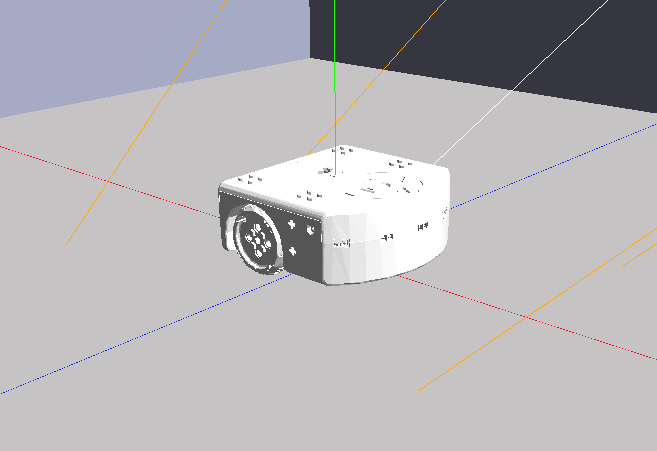
\includegraphics[width=\textwidth]{./title}
  \end{center}
\end{titlepage}

\clearpage


\includegraphics[width=\textwidth]{./Declaration_of_authonomy.pdf}
\clearpage

Management Summary
\clearpage

\tableofcontents
\clearpage

\chapter{Introduction}

\chapter{Environment}

\section{Three JS}

\texttt{three.js} is a 3D library for \texttt{JavaScript} which uses a default \texttt{WebGL} renderer. It allows the user to display, create and animate 3D computer graphics in a web browser. Its basic rendering pipeline is as follow :
\begin{center}
  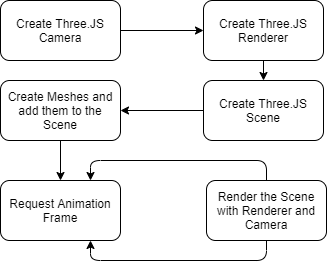
\includegraphics[scale=0.5]{./basic_threejs_rendering}
\end{center}

Every \texttt{three.js} application is composed of at least one \texttt{Camera} element, a \texttt{Renderer} element and a \texttt{Scene} element. The different meshes are added to the scene and this scene along with the camera are rendered using the method 
\texttt{requestAnimationFrame} from \texttt{three.js} on the renderer element. 
%% TODO : ADD A BIT OF TEXT

\chapter{Thymio}
\section{What is Thymio} 

Thymio is an educational robot that aims at improving early education (starting in primary school) in STEM (Science, Technology, Engineering and Mathematics),
computational thinking, base computer science and researching the acknowledgement by kids of robots in their learning environment.
The project also had technical aims, such as how to provide hardware modularity, fast reaction time amid perception and action,
clear internal communication bus in a user-friendly way and streamline development for group robot, this includes direct changes to the robots’ programs and parallel debugging wirelessly, 
transparently and cheaply.\\

The Thymio project is based on a collaboration between the MOBOTS group from the Swiss Federal Institute of Technology in Lausanne (EPFL) and the Lausanne Arts School (ECAL).
MOBOTS being the Miniature Mobile Robots Group, they are mainly focused around system design for small robots of the kind. It started with a strange-looking pile of components, 
that were assembled on any kind of support and hold the name of “Monsieur Patate” (Sir Potato), most likely due to its appearance, 
that saw life during the first workshop between the two contributors. After what the first “Thymio” was developed, 
it was a four-block robot that could be self-assembled, but not self-programmed as it was coming with pre-programmed behaviours. 
It was used as a user study to gather feedback from clients to know what features needed to be implemented on the Thymio II.\\

\begin{center}
  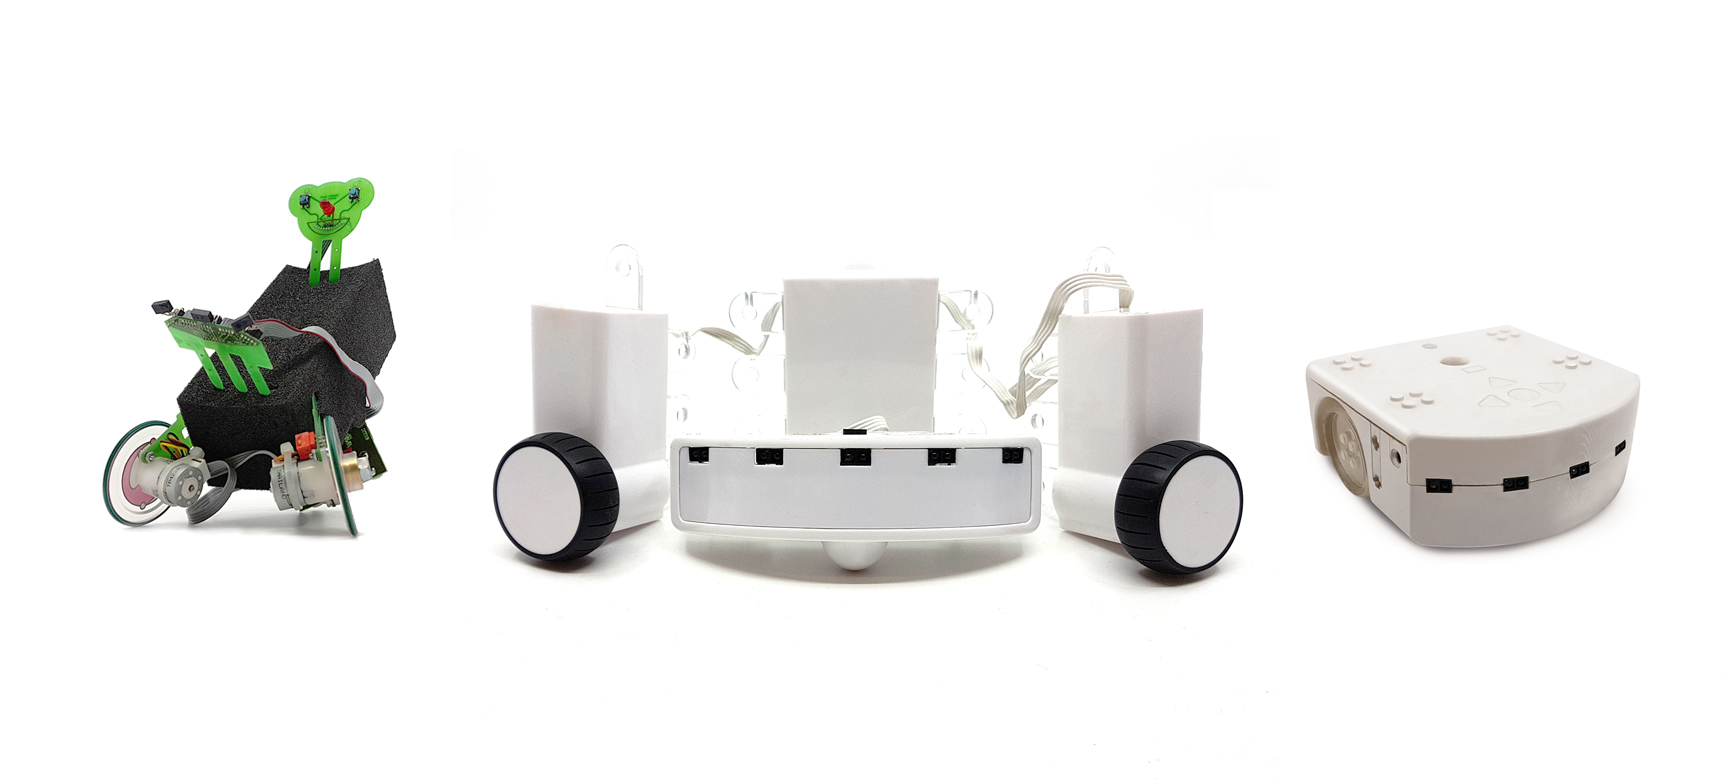
\includegraphics[width=\textwidth]{prototype_thymio_old}\\
  From left to right, "Monsieur Patate", Thymio, Thymio II
\end{center}

The result is a robot with a complex and complete set of sensors and actuators. 
The National Centre for Competence in Research (NCCR) Robotics research program supported the development of the robot whereas Mobsya, 
a non-profit organization that creates a robot, software, and educational activities to broaden young people's mind about technology and science, 
oversees the production, distribution, and communication of said robot. 
Every step of the Thymio project is open-source and has a non-profit aim to enhance the quality of it with the user's project and research, 
and reduce the cost and augment the lifetime for educational platforms and materials.

\begin{center}
  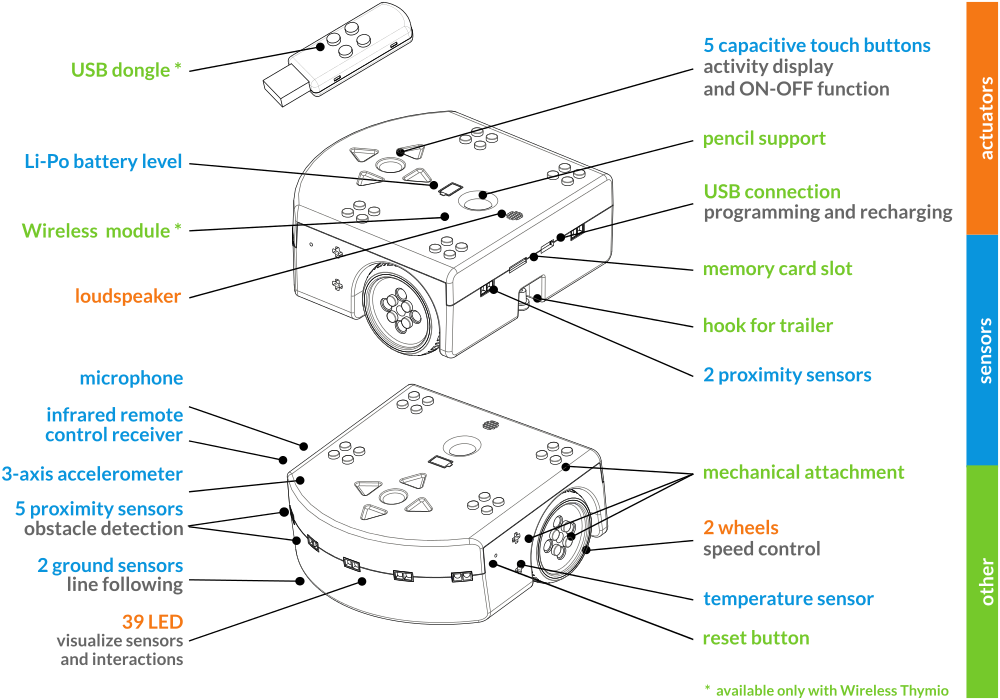
\includegraphics[width=\textwidth]{Wireless-thymioII-sensor-actuator-color-en}\\
  Thymio II sensor and actuator
\end{center}

\section{How does it works \label{howdoesitworkref}} 

As seen in the figure above there exist two Thymio models, Thymio and Wireless Thymio. 
The difference between them lies in the ability of the second one to be programmed wirelessly, 
as its name suggests. To begin the creation of a program for the robot there exist two possibilities.
The first one, and the most common one for the public is done by using the software Aseba and a connected Thymio. 
In this case, the robot needs to be plugged in via USB cable or USB dongle (possible only if it is the Wireless Thymio) and powered on. 
Then the software can be used to connect to said robot and start to program in one of the four different programming languages, 
that are: VPL, Blockly, Aseba, and Scratch. Once the program is ready and sent to the robot it will be available to play. \\

The second option is to use the work-in-progress Thymio Suite version. 
This software doesn’t require a Thymio robot to be connected physically (or wirelessly) at all times as it has its own simulator built-in. 
The four said languages are still available, and one need to be chosen. 
After what comes the choice of connecting a physical Thymio or starting a simulation to emulate the programmed behaviour.
A more detailed section on the four differents programming languages can be found in the section \ref{fourlanguages} at the page \pageref{fourlanguages}.

\chapter{Requirements Documentation}
\section{Vision}

A start-up from the EPFL has developed a robot, the Thymio robot or Thymio II, that promotes the programming and robotic activities among children. 
To feed program to the robot, a software has been developed, it integrates the four following programming languages: 
\begin{itemize}
  \item VPL
  \item Blockly4Thymio
  \item Aseba
  \item Scratch
\end{itemize}

The project Web Simulation of a Thymio robot is aimed to create a simulator for the Thymio II so as to allow people to see their programmed behaviour directly.

\section{Goals}

This aim has been split into 6 different defining goals in order to create this application.
\begin{center}
  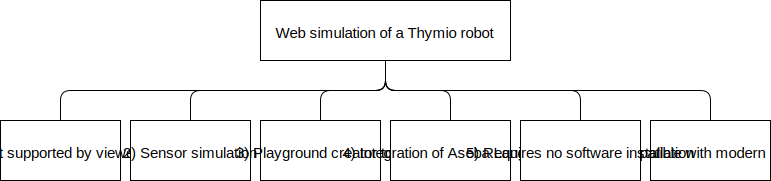
\includegraphics[width=\textwidth]{./goals}
\end{center}

\section{System Context}
%%\section{Requirements}
\section{Risk Analysis}
In order to carry out the project successfully, we must consider the following possible complications. The possible complications are on one hand assessed according to their impact and on the other hand according to their likelihood to occur. 
Thus, we obtain a predictable risk factor that allows us to have an overall view and take preventive measures if necessary.

\begin{center}
  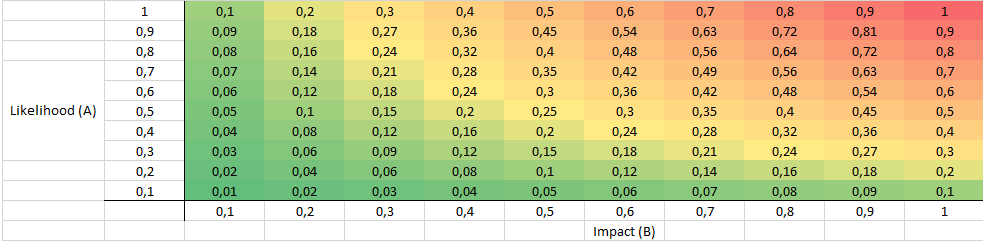
\includegraphics[width=\textwidth]{./risk-matrix}\\
  Risk Matrix
\end{center}

\begin{tabular}{p{2cm} p{2cm} p{2cm} p{2cm}}
  Event & Likelihood (A) & Impact (B) & Risk Factor (A*B) \\ \hline
  Financial issues & 0 & 1 & 0 \\
  Collisions not implemented & 0.3 & 0.6 & 0.18 \\
  Behaviour pipeline not working & 0.4 & 0.9 & 0.36 \\
  Playground creator not working & 0.4 & 0.6 & 0.24 \\
\end{tabular}

\section{Stakeholder Descriptions}
\textbf{Product Owner}
Flückiger Quentin flucq1@bfh.ch \\
\textit{Interests}:
\begin{itemize}
  \item The product owner wants to satisfy the customer.
\end{itemize}


\textbf{Development Team}
Flückiger Quentin flucq1@bfh.ch \\
\textit{Interests}:
\begin{itemize}
  \item The development team wants to develop a usefull application for the customer.
\end{itemize}

\section{User Stories}
\textbf{\large Users User Stories}\\
\textbf{As} a user, I want to upload an .aesl file, so that I can witness the simulated behaviour. \\
Description:\\
The user wants to upload an .aesl file to see the programmed behaviour simulated.
Success:\\
\begin{itemize}
  \item The simulation works.
\end{itemize}
Failure:\\
\begin{itemize}
  \item The .aesl file doesn't contain a program.
  \item The .aesl file contains behaviour not included in the simulator.
\end{itemize}


\textbf{As} a user, I want to create a simple testing environment, so that I can diversify the experiences. \\
Description:\\
The user wants to create home made playground with a simple playground creation tool.
Success:\\
\begin{itemize}
  \item The playground was successfully created and saved.
\end{itemize}
Failure:\\
\begin{itemize}
  \item The created playground isn't saved properly.
  \item The user encounters trouble while creating the playground, be it meshes creation or placement.
\end{itemize}


\textbf{As} a user, I want to use the application without having to install anything, so that the application can be accessed easily. \\
Description:\\
The user wants to access and use the application without installing anything.
Success:\\
\begin{itemize}
  \item The use can start the application directly in his browser.
\end{itemize}
Failure:\\
\begin{itemize}
  \item The webserver isn't accessible.
\end{itemize}

\section{Use Cases Model}

\textbf{Use Case: }Access the application \\
\textbf{Primary Actor: }User \\
\textbf{Stakeholders and Interests: }User: Wants to access the application through a web browser. \\
\textbf{Preconditions: }User has access to the bfh network. \\
\textbf{Success Guarantee (Postconditions): }The user can access the application via a modern web browser. \\
\textbf{Main Success Scenario: } 
\begin{enumerate}
  \item User start web browser.
  \item User navigate to website address.
\end{enumerate}
\textbf{Extensions: } 
\begin{enumerate}
  \item 
  \begin{enumerate}
    \item No available internet connection.
  \end{enumerate}
  \item 
  \begin{enumerate}
    \item Not logged in the bfh network.
    \item Web Server currently offline.
  \end{enumerate}
\end{enumerate}
\textbf{Special Requirements: }Modern web browser compatibility. \\
\textbf{Technology and Data Variations List: }- \\
\textbf{Frequency of Occurrence: }Could be nearly continuous.\\
\textbf{Open Issues: }- \\
\\
\textbf{Use Case: }Interprete .aesl file \\
\textbf{Primary Actor: }User \\
\textbf{Stakeholders and Interests: }User: Wants to load .aesl behaviour file to be translated and simulated. \\
\textbf{Preconditions: }User has a .aesl file containing behaviour code for Thymio. \\
\textbf{Success Guarantee (Postconditions): }File is correctly compiled, and simulation simulate expected behaviour. \\
\textbf{Main Success Scenario: }
\begin{enumerate}
  \item User access the website.
  \item User input a .aesl file.
  \item System control file integrity.
  \item System compile file to \texttt{JavaScript} code that can be run as behaviour.
  \item System run given program.
\end{enumerate}
\textbf{Extensions: }
\begin{enumerate}\addtocounter{enumi}{1}
  \item 
  \begin{enumerate}
    \item File too large for application.
  \end{enumerate}
  \item
  \begin{enumerate}
    \item System signals error and reject file because not conform to awaited structure.
  \end{enumerate}
  \item 
  \begin{enumerate}
    \item System signals error while compiling file.
  \end{enumerate}
\end{enumerate}
\textbf{Special Requirements: }- \\
\textbf{Technology and Data Variations List: }- \\
\textbf{Frequency of Occurrence: }Very often. \\
\textbf{Open Issues: }- \\
\\
\textbf{Use Case: }Change playground \\
\textbf{Primary Actor: }User \\
\textbf{Stakeholders and Interests: }User: Wants to change the rendered playground. \\
\textbf{Preconditions: }User has access to the bfh network. \\
\textbf{Success Guarantee (Postconditions): }The playground is changed accordingly the whishes of the user. \\
\textbf{Main Success Scenario: }
\begin{enumerate}
  \item User access the website.
  \item User chooses the wanted playground.
  \item System load wanted playground.
\end{enumerate}
\textbf{Extensions: }
\begin{enumerate}\addtocounter{enumi}{1}
  \item 
  \begin{enumerate}
    \item The input file is not from the right file extension. 
  \end{enumerate}
  \item 
  \begin{enumerate}
    \item Fail to load playground because file not conform to awaited structure.
    \item Internal error when playground was loaded.
  \end{enumerate}
\end{enumerate}
\textbf{Special Requirements: }- \\
\textbf{Technology and Data Variations List: }- \\
\textbf{Frequency of Occurrence: }Often. \\
\textbf{Open Issues: }- \\
\textbf{Sequence diagram: } \\
\begin{center}
  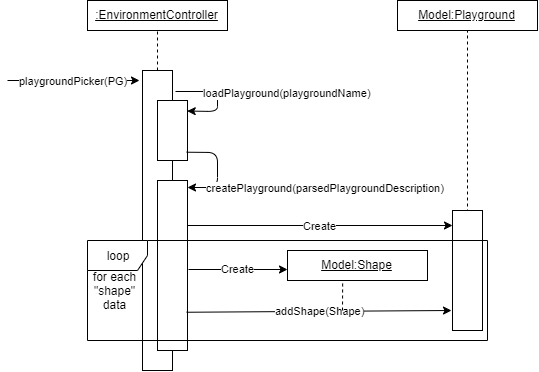
\includegraphics[scale=0.7]{./loadPlayground_sd}
\end{center}


%%Use case diagram

\chapter{Architecture}
%% Domain class diagrams, Domain model, Package diagram, Sequence diagram, System sequence diagram

We decided to divide the architecture into two different parts. One for the simulation side and the other one for the customization, although they are very similar there are still some differences that push us to look at them with two different angles. Both are build based on a Model View Controller system where the elements of the playground, be it a wall or the Thymio robot, are models and the page is seen by the user is the view. This view registers user inputs and transmits them to the controller. 

As said we have split the architecture, bellow is a graphic representing the architecture for the simulator. We can see the Model View Controller and a second component which is the interpreter, 
that is singular to the simulator page. Its role is to test the integrity of the file given as input through the controller and compile it into \texttt{JavaScript} code for it to be used as behavior code for the Thymio Model.

\begin{center}
  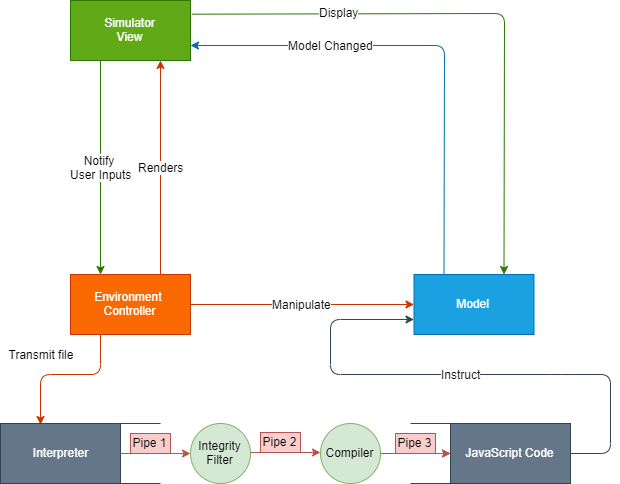
\includegraphics[width=\textwidth]{./architecture_proposal-Page-1}
\end{center}

And here is the second Model View Controller responsible for the playground customization, its architecture is the same as the other one except it doesn't implement an interpreter.
\begin{center}
  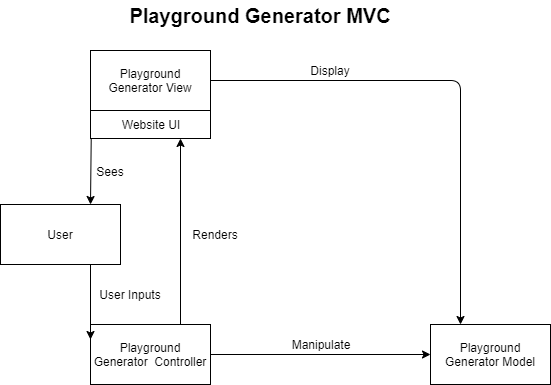
\includegraphics[width=\textwidth]{./architecture_proposal-Page-2}
\end{center}
%% TODO : Add text about different elements and transition, link it with current code


\chapter{What already exist} 

There exist two possibilities to simulate the behavior of a Thymio II Robot on a computer. 
The first one is through the Thymio Suite application developed by the creator of Thymio. 
It is an application that regroups multiple features such as coding the robot in one of the four available languages, 
uploading the program to a real robot or simulating its behavior via a simulator developed in the programming language C++. 
This simulator allows one to load a playground among multiple pre-set and run the coded program for the robot.

\begin{center}
  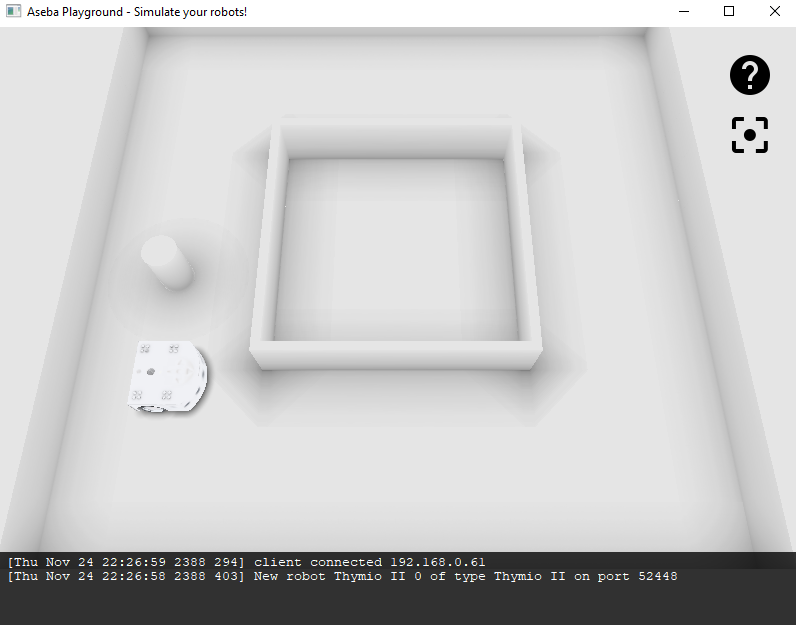
\includegraphics[width=\textwidth]{./suite_simulator}
\end{center}

The other option is to use WeBots, which is an open-source 3D robot simulator for industry, education and research purpose. 
It has been developed in 1996 at the Swiss Federal Institute of Technology in Lausanne since then it became a property license software of Cyberbotics in 1998, 
and in December 2018 was lastly released under the free and open-source Apache 2 license.
WeBots is a very powerful software that can do a lot of things, and one of these things is an accurate Thymio II model with almost all its sensors and actuator. 
The two Aseba Studio and VPL for Thymio can be directly connected to the software and its simulated robot. 
The specification and usage can be found on their website with the following link \href{https://www.cyberbotics.com/doc/guide/thymio2#mosybas-thymio-ii}{WeBots Thymio} .
%% TODO : Add more text

\chapter{Our Approach}

\section{Base Development}

The first steps were to learn how to use the \texttt{threejs} library and thus we integrated the needed code directly onto some .html file, which was not very efficient for a big application but was okay to test the functionalities. 
At that time, we looked for some useful methods that we would need later on, such as the way to resize the window and its content. Another functionality added at this period was the controls of the camera, that comes from the OrbitControls.js file and allows the creation of an OrbitControls object which let the user move the camera, rotate it and zoom with the mouse.
Afterward, we implemented method to create different Shapes with more ease for a larger application. We then moved the scripting part outside of the html and inside different \texttt{JavaScript} file as it was not convenient to have all the code into one single html file.


\section{Model View Controller}

Registration of buttons,
What happens when a button is clicked.
\begin{center}
  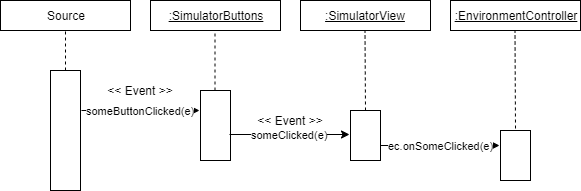
\includegraphics[width=\textwdith]{./button_mvc}
  \label{button_mvc}
\end{center}

\section{WebServer \label{webserver}}
Regarding the goal number 5, Require no software installation, we decided to use a webserver in order to access the application. At first we choose the IIS Manager that is built in with Windows 10, 
we followed the steps in this tutorial video in order to configure IIS: \url{https://www.youtube.com/watch?v=rPRLe7QeVHM} .

Then we had to open the port in order to access it from within the LAN.
\begin{enumerate}
  \item Open the windows Firewall, click on Inbound Rules and New Rule. This will open the New Inbound Rule Wizard.
  \item Select the desired type, Port, click next.
  \item Choose TCP and specify the port used, here 80, click next.
  \item Select Allow connection, click next.
  \item Select all three profile options, click next.
  \item Add a Name and a description to this rule, click finish.
\end{enumerate}

\textbf{Additional setup}\\

It was needed to create a web.config file and add a few file extension so that the .mtl and .obj would still be able to load. 
Otherwise we encountered an error of the type "Failed to load resource: the server responded with a status of 404 (Not Found)." 
The text that needed to be added to the web.config file is the following : \\
\begin{lstlisting}[language=XML, basicstyle=\ttfamily\small]
<?xml version="1.0" encoding="UTF-8"?>
  <configuration>
    <system.webServer>
         <staticContent>
           <remove fileExtension=".mtl" />
           <mimeMap fileExtension=".mtl" mimeType="text/plain" />
           <mimeMap fileExtension=".obj" 
              mimeType="application/octet-stream" />
         </staticContent>
    </system.webServer>
</configuration>
\end{lstlisting}

Unfortunately, after implementing the new MVC architecture for our application we encountered an issue where the application wasn't able to locate some \texttt{JavaScript} file and giving the following error message in the console : 
\texttt{javascript file not found on server, net::ERR\textunderscore ABORTED 404 (Not Found)} .  After a while of debugging and asking questions to persons who could know the issue, 
we decided to move away from ISS Manager as our knowledge of this software is too small and the time needed to acquire this knowledge wasn't worth the effort. 
The alternative solution we came up with was to use XAMPP, we managed to push the same version of the application without any problem and without having to do anything special. So we decided to go forth with XAMPP.

\section{Playgrounds}

We decided to create three different build-in playgrounds for the application. A basic, with four walls and a square plane. A borderless, composed of a track that leads out of the octagon plane. And one with multiple obstacle, walls and a track. 
Each on of them would be composed of one \texttt{Group} element that is filled with different meshes created from the previously implemented method found in the \texttt{GeometricalMeshes.js} file.

We decided to enhance the the amount of different meshes and thus added an algorithm to create tracks. There was two steps for the algorithm to create tracks, the first one was to compute a simple line between two points. 
But the result was too thin and therefore a better solution was found.
The second iteration for this alogrithm takes an array of points, those points are of type Vector3 so as to register the three coordinates, and compute 
a new Vector3 that holds the resulting vector position of the next point minus the current point. The x and z values of this vector are then used 
as the center to position a box object, which represent the track, and then it is aligned to this vector.
\begin{lstlisting}[language=JavaScript, basicstyle=\ttfamily\small]
  for (let i = 0; i < points.length-1; i++) {

    const trackWidth = new THREE.Vector3().copy(points[i+1]).sub(points[i]);
    const track = new THREE.Mesh(
      new THREE.BoxGeometry(trackWidth.length(), TrackHeight, TrackDepth),
      material
    )

    track.position.x = points[i].x + trackWidth.x/2;
    track.position.z = points[i].z + trackWidth.z/2;
    track.quaternion.setFromUnitVectors(new THREE.Vector3(1, 0, 0), 
      trackWidth.clone().normalize());
    container.add(track);      
  }
\end{lstlisting} 

We decided to load only once the Thymio model, as it takes in average 500ms to 1'000ms to load it, and we encountered some issues where the model would not load everytime when we would change the playgrounds.
Therefore we reset it's position and rotation whenever we change the playground, or if a position is given in the playground.json data file, the Thymio is moved to the wanted position.

Thinking about the creation of playground we decided to change how the playgrounds data were recorded and instead of having them as \texttt{JavaScript} file, we moved them all into a \texttt{JSON} file. So later on it would not require more work to load a 
customized playground. To do so we open and read a \texttt{JSON} file of a given name, and then skim through the \texttt{JSON} file and create the Shapes accordingly of the data. Bellow an example for the boxes.
\begin{lstlisting}[language=JavaScript, basicstyle=\ttfamily\small]
  if (file.boxes) {
    for (const boxRecord of file.boxes) {
        var box = new Box(boxRecord.name, boxRecord.props);
        playground.addShape(box);
    }
  }
\end{lstlisting} 

Unfortunately we found later on that \texttt{threejs} has a built in function that translate a ThreeJS Object into a \texttt{JSON} file element, and inversely. But we are still using the solution we developed.

\section{Interpreter}
The interpreter found that compile/translate .aesl file into another programming language is the one used in the Thymio Suite application, its source code can be found in the following repository \href{https://github.com/aseba-community/aseba/tree/master/aseba/compiler}{Aseba git}.
Unfortunately, it is a C++ one, so we had to understand it and find a way to either use it and then use a C++ to \texttt{JavaScript} interpreter, or translate the compiler from \texttt{C++} to \texttt{JavaScript} by hand.
We decided to translate the already existing one from \texttt{Aseba} and started by the compiler. After looking at his behaviour we recognize how it was built and separated,
then came the time to translate it to \texttt{JavaScript}. First thing first it creates multiple maps of variable, constant and events that need to be rebuild with each call to the compiler in case the previous ones produced errors.
Afterwhat comes the tokenization of the source file, which consist of creating Tokens with the position of the element, its type in the environment, and its value if provided. Then this tokenized source is parsed into Nodes, 
which are expanded and type checked. Once the program is checked, it is emited as a first bytecode output and then this bytecode is linked creating the final program.

Here is a sequence diagram of the compilation of a file.
\begin{center}
  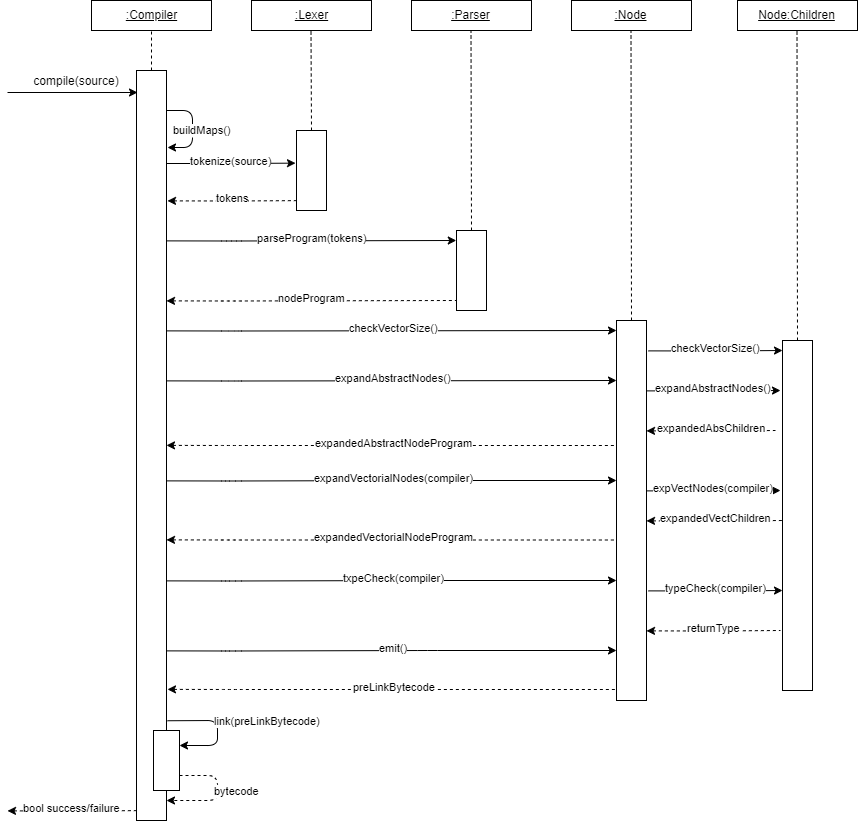
\includegraphics[width=\textwidth]{./compiler_sequence_diagram}
\end{center}
%% TODO : ADD MORE TEXT

\subsection{Tokenize}

To tokenize the source file we skim through the document and switch depending on the value of the character, we have basically five categories for this switch.
The first one are the tokens which require only to read one character, such as \texttt{)}, \texttt{,} those can directly be given their type. Next are the comments, the comment block ,\texttt{\#* ... *\#}, or the simple line comment ,\texttt{\#}. For the block comment,
we run through the source in search of the \texttt{*\#} character association that marks the end of the comment block, throwing an error if not found. The third category encompass the cases that require one character look-ahead, such as when we found
the character \texttt{+} is it a simple \texttt{+} or \texttt{+=} or even \texttt{++} ? The fourth is almost the same but with two characters look-ahead, such as \texttt{<}. The fifth category, and the default case of this switch, is the one where the amount of look-ahead needed is not defined.
In this category fit the numbers and the strings, which are found using a regex as replacement of the \texttt{C++} method \texttt{is\textunderscore utf8\textunderscore alpha\textunderscore num()}, which controls that the element is either a letter or a number. Bellow is 
the code for this regex.
\begin{lstlisting}[language=JavaScript, basicstyle=\ttfamily\small]
  isAlphaNumeric(ch) {
    return ch.match(/^[a-z0-9]+$/i) !== null;
  }
\end{lstlisting}  
We have to be wary of one point when using this method, and it is that if the \texttt{ch} parameter is not a string, then it will throw an error. Coming back to the switch we first test if the chain of character is a number by combining regex and looking for multiple characters.
If it is not the case we check wether or not its value is the same as one of the given keywords, such as \texttt{when} or \texttt{const}. And if none of the keywords match it is labeled as a string literal and given the value of the chain of characters. Here we encountered a probleme 
of language between C++ and \texttt{JavaScript}, as the type of the token is given with an enum in C++, and they don't exist in \texttt{JavaScript} so we had to find a workaround to this language incompatibility. We used the Object method \texttt{freeze()}, which prevents the modification of existing property attributes and the addition of new ones, 
and still had to give a value to each properties.

\subsection{Parser}

%% TODO : Write what we have done and so and so
Once the source file is tokenized we can parse it into a three. To do so we translated the needed part of the three from \texttt{Aseba} in C++ to \texttt{JavaScript}.


\section{Phyisics}

Adding physics to allow collisions between the robot and the different objects. Trying to use Physijs, source code can be found in the following repository \href{https://github.com/chandlerprall/Physijs/wiki/Basic-Setup}{Physijs git}, 
but with the architecture of our application, we encounter a problem due to the fact we are adding THREE.Object3D instead of basic mesh and Physijs works only with a fixed amount of meshes. A solution would be to not use Physijs as we need it only for the Thymio,
and instead, shoot rays from the robot and check for collisions this way, as only Thymio needs to move and stop upon collisions.

\section{Sensor and Actuator}

We represented the five buttons that sit on top of the Thymio directly in the UI and did not give the possibility to interact with the modelized ones. We wanted to create a Directional Pad style group of buttons such as in the first image bellow, 
but ended with the second image, which is less nice, due to the time needed to make it perfect. All the buttons work as the previously explained sequence diagram on page \pageref{button_mvc}.
\begin{center}
  \begin{tabular}{c c}
    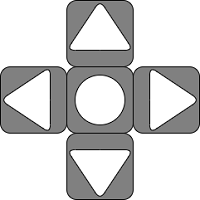
\includegraphics{dpad} & 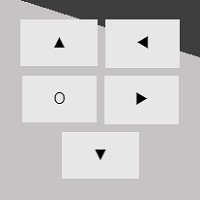
\includegraphics{fake_dpad}
  \end{tabular}
\end{center}

A Thymio robot moves in according with two motors, one for its right wheel and one for its left wheel. They have a value for the output power between -500 and 500, minus meaning the motor powers the wheel in the opposite direction. 
And those two motors can only output power in a straight line, forward / backward. Bellow are three representations of the expected movements of a Thymio. The yellow arrow is the power for the left motor, the blue arrow is the power for the right motor, 
and the green arrow is the final vector movement for the robot. On the first representation, the power of the two motors are the same, both in value and direction, thus the final vector is simply the same as either one of the two.
On the second one, the value of the power for both motors is still the same but their direction is opposite, hence the final vector is a circle because the robot will turn on itself.
And finally, the third representation shows the resultant vector when the value is not the same but the direction is.
\begin{center}
  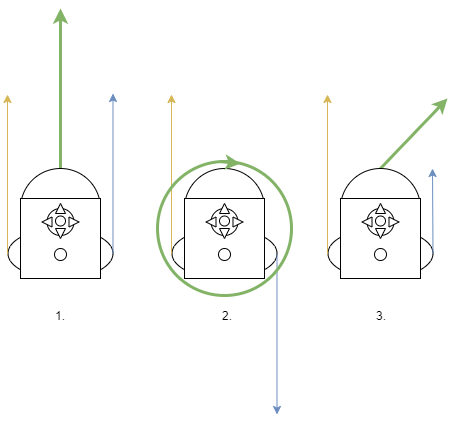
\includegraphics[scale=0.8]{./thymio_move}
\end{center}

It was complex to convey the way the Thymio robots move onto this application as we move models and don't physically power motors. To achieve the same behavior we decided to use some trigonometry and a few tricks.
The method that moves the robot is called only within the \texttt{render()} method from the main View, and thus every time the scene is being rendered we move the robot accordingly to the value of the motor. 
Those values are set using the \texttt{setMotors(left, right)} method. The \texttt{move()} method, the one that computes the movement of the robot, is split into four categories depending on the values of the motors. 

The first category is when both motors have the same power in the same direction, therefore the resulting position change for both x and z coordinate is computed using the \texttt{getDirection()}, which returns 
a Vector3 representing the direction the robot is facing, a predefined speed variable and the power given to either of the motors.
\begin{lstlisting}[language=JavaScript, basicstyle=\ttfamily\small]
  getDirection() {
    var direction = new THREE.Vector3();
    return this.object3D.getWorldDirection(direction);;
  }
\end{lstlisting} 
\begin{lstlisting}[language=JavaScript, basicstyle=\ttfamily\small]
  this.object3D.position.x += 
    this.getDirection().x * this.speed * this.rightMotor;
  this.object3D.position.z +=
    this.getDirection().z * this.speed * this.rightMotor;
\end{lstlisting}  
\begin{center}
  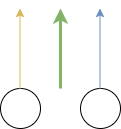
\includegraphics[scale=0.8]{./move_spsd}
\end{center}

The second option is when the value of the left motor is bigger than the right, regarding the direction. Alternatively, the third option is the same but when the value of the right motor is bigger than the left.
\begin{center}
  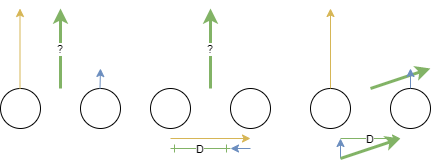
\includegraphics[width=\textwidth]{./move_dp}
\end{center}
In this case, we calculate the difference D of power between the two motors, the biggest minus the smallest, and then we use trigonometry to find the angle between the power of the motor and the resulting vector of the addition of the power of the motor and the difference D.
This angle is then used as a parameter to rotate the model around the y-axis, to smooth things we multiply it by a variable turnSpeed.  
\begin{lstlisting}[language=JavaScript, basicstyle=\ttfamily\small]
  this.object3D.rotateY(
    -(Math.atan(delta/Math.abs(this.leftMotor))*this.turnSpeed)
  );
\end{lstlisting} 
The resulting change in position is computed the same way as for the first category. It might be more relevant to use the norm of the resulting vector 
found earlier to have a more accurate speed.

The fourth category happens when both power values are the same but in a different direction. In this case, we rotate the robot on itself around the y-axis according to either of its motor speed.
\begin{center}
  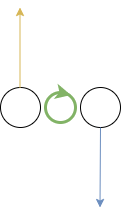
\includegraphics[scale=1]{./move_spdd}
\end{center}

However this algorithm has flaws such as when the power of one motor is 0 the robot should be rotating on itself with said motor as anchor point, but instead it rotate and moves in the direction of the second motors direction.

To determine if a collision occurs between the robot and one of the element of the environment we decided not to use an external phyisic but instead we throw raycast from various position 
%% TODO : Proximity sensors
%% TODO : Lights
%%How they work in real life, what do they output, what do they return as value, and how they work in the application.

\section{Customize playgrounds}

The creation of a customize playground that can be used later on in the simulation part of the application takes place on a different page. On this page, we keep the same architecture as for the simulation but we change the \texttt{Controller} and the \texttt{View} elements 
and don't add the compilation part. Thus most of the changes and logic come from the \texttt{CreatorController.js} file. We reflected  on how the data of the playground would be carried, or kept, and used in the simulator. Thus we had multiple options,
such as using a database to store every customed playground so that they would all be available with the application. Or to download  them locally as a file on the user's computer. We went with the latest option as we previously prepared the program to load playgrounds from \texttt{JSON} files.
Saving the playground data is done in four different steps, bellow a sequence diagram of the process.
\begin{center}
  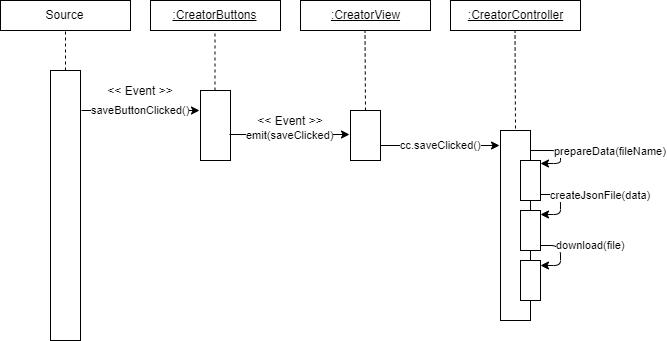
\includegraphics[width=\textwidth]{./savepg_sd}
\end{center}

First, once the event that the save button has been pressed the application will open a \texttt{prompt} window in which the user will specify the file name. Then the data that composed the customized playground are behing separated into different array based on their \texttt{className} property. 
Once every shapes contained in the cusomized playground have been gone through and categorized we create the final \texttt{JSON} file, it is created by using the \texttt{forEach} method of \texttt{JavaScript} array and writing the name of the mesh and it's properties. 
Finally the file is downloaded on the user's computer and the process ends.

%% TODO : Add part of json file with data as example

It was needed to add a few more controls over the scene in order to increase the ease of use and the possibilities of creation. The camera controls need to be enabled so that the user can navigate through the scene but once he chose the spot he wants 
the mesh to be at he needs to deactivate those controls with the \texttt{shift} key, and enabled them back with the same key. We decided to add three other controls. The first is the use of the \texttt{Esc} key to cancel the current mesh positioning, it removes the current placeholder from the scene. 
The second and third are linked one to the other, it's the use of the \texttt{ctrl-Z} and \texttt{ctrl-Y} logic. To do so we create two different arrays, one with the current meshes in the scene and the other one with the removed meshes, which operate as \texttt{LIFO} Queue.
However we test that the length of the respective array is legal to perform the action and if the current shape the user is creating is from the type \texttt{Tracks} then we apply another logic, which removes/reinserts the last point of the track.
There are three different shapes at the user's disposal and two types of grounds. A ground element will always be needed to save the current playground, otherwise, an error occurs. The two types of grounds are a simple rectangle and an octagon, with a set of properties. 
Changing the properties will not change the mesh in real-time, but once the button \texttt{Generate Ground} is pressed it will remove the previous ground and add the new one. The creation of boxes and cylinders takes part in two steps. 
During the first step, the user will choose the properties, such as \texttt{width}, the \texttt{length}, the \texttt{height}, the \texttt{color} and the \texttt{rotation} for the box, and then by clicking the \texttt{Generate} button of said shape, 
a placeholder of the shape will be instantiated and it will follow the movements of the mouse while rounding its position to fit into the square represented by the \texttt{THREE.GridHelper} element. 
\begin{lstlisting}[language=JavaScript, basicstyle=\ttfamily\small]
  this.rollOverMesh.position.divideScalar( 1 ).floor()
    .multiplyScalar( 1)
    .addScalar( 0.5 );
\end{lstlisting} 
Then the user has multiple-choice, either click to fix the mesh onto the scene, or the properties didn't fit what he wanted so he would click once more on the \texttt{Generate} button with the new properties, 
or cancel the action with the \texttt{Esc} key. 
To lay Tracks we needed to create one more step as the mesh is composed of multiple points, those points are laid the same way as a \texttt{Box} mesh would but they are added to an array that stores the position of those points. 
Once the track is finished and upon clicking on the \texttt{Generate Track} button the points placeholders will be removed and a track passing through the wanted positions will be computed by looping through the points array and feeding the property element of track with the position of \texttt{X} and \texttt{Z} of each points.
\begin{lstlisting}[language=JavaScript, basicstyle=\ttfamily\small]
  this.points.forEach(pt => {                      
    this.props.points.push({
      positionX : pt.position.x,
      positionZ : pt.position.z
    });
  });
\end{lstlisting} 
However, the algorithm that tracks the movement of the mouse and changes the position of the temporary mesh is not optimized and will slow down the application drastically. Unfortunately we don't know which part of the algorithm has to be optimized.


\chapter{Results}



%%\section{Usefull latex commands (to be deleted later on)}
%%\lstset{language=JavaScript}
%%\begin{lstlisting}[basicstyle=\ttfamily\small]
%%  function generateBox(color, width, height, depth){

%%    var geometry = new THREE.BoxGeometry( width, height, depth );
%%    var material = new THREE.MeshPhongMaterial( { color : color} );
%%    var box = new THREE.Mesh( geometry, material );
                
%%    return box;
%%  }
%%\end{lstlisting}
%%For that we read the article book of \cite{Jerald:2015:VBH:2792790}
%%which is very interesting, much more than the article
%%\cite{Diniz:2017:UGO:3100317.3100324}
%%

\chapter{Conclusion and future work}

Translate rest of functionality from c++ parser and co, add more sensors and actuator (sounds, pen and co)
Better sensors
Architecture too heavy and restrictive
Very difficult to understand a whole C++ application and select the part needed to be translated
Interpreter taking way more time than imagined

\appendix

\chapter{The different programming languages \label{fourlanguages}} 
\section{VPL}

One of the four different possibilities to program the Thymio is by using the visual programming language, or VPL, 
developed by the creator of Aseba. A visual programming language is an abstraction of the more common way to program. 
It is based on the manipulation of program elements graphically that can be manipulated following some spatial grammar to create a program. 
VPLs are based on a set of entities and relations, whereas most of the time entities are represented by boxes, 
or other graphical objects, and relations by simple arrows. They can be categorized into icon-based, 
form-based and diagram-based languages depending on the extent of visual expression inside of it. 
The use of visual programming languages can be found in multiple areas, such as the game engine “Unreal Engine 4” where their system of Blueprints is created upon a node-based VPL, 
or “Microsoft SQL Server Integration Services”. This abstraction allows easier access for neophytes, 
for example using graphic elements such as blocks, forms, diagrams, and others reduce drastically, if not eliminate, the syntactic errors made by the user.\\

In the case of the VPL developed by Aseba’s team, and the one we are mostly interested in, we have a programming language based on two types of blocks: Event blocks and Action blocks. 
From those two are built the seventeen, respectively eleven event blocks and six action blocks, entities. 
One of the main goals of VPL for Thymio was to let people who cannot yet read the ability to start programming and discover this world.\\

\begin{center}
  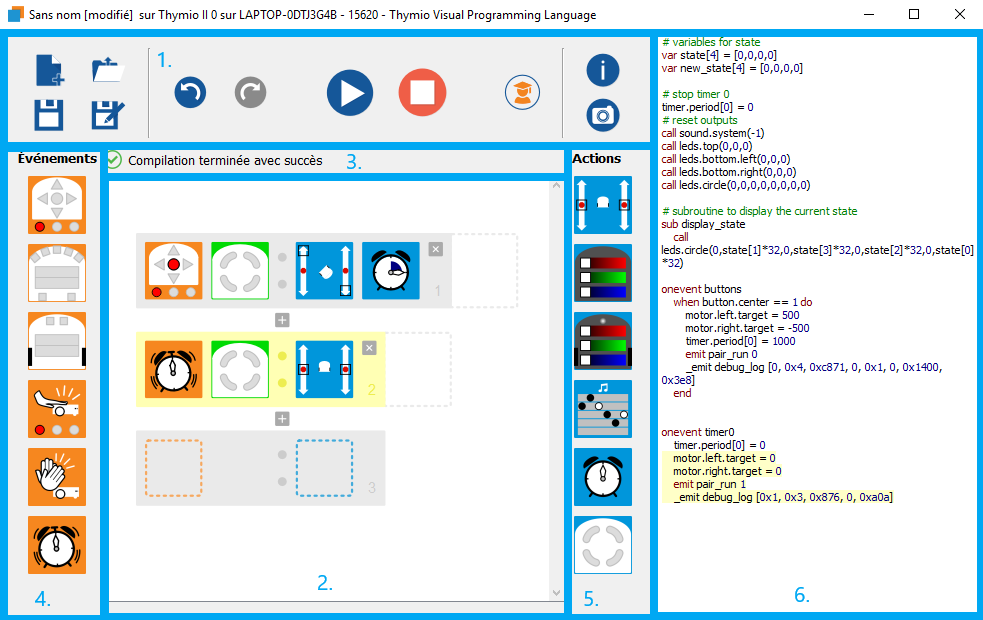
\includegraphics[width=\textwidth]{./VPL/Thymio_VPL_window}\\
  Thymio VPL Event and Action blocks
\end{center}

To begin creating a program follow the first steps described in the section \ref{howdoesitworkref} at the page \pageref{howdoesitworkref}. 
Once the VPL option has been chosen and the Thymio Visual Programming Language window appears we are ready to go. 
The window is split into six different regions with each of their purposes.
\begin{enumerate}
  \item A tool bar
  \item A programming window
  \item Console messages
  \item The event blocks
  \item The action blocks
  \item The program translated into AESL
\end{enumerate}

\begin{center}
  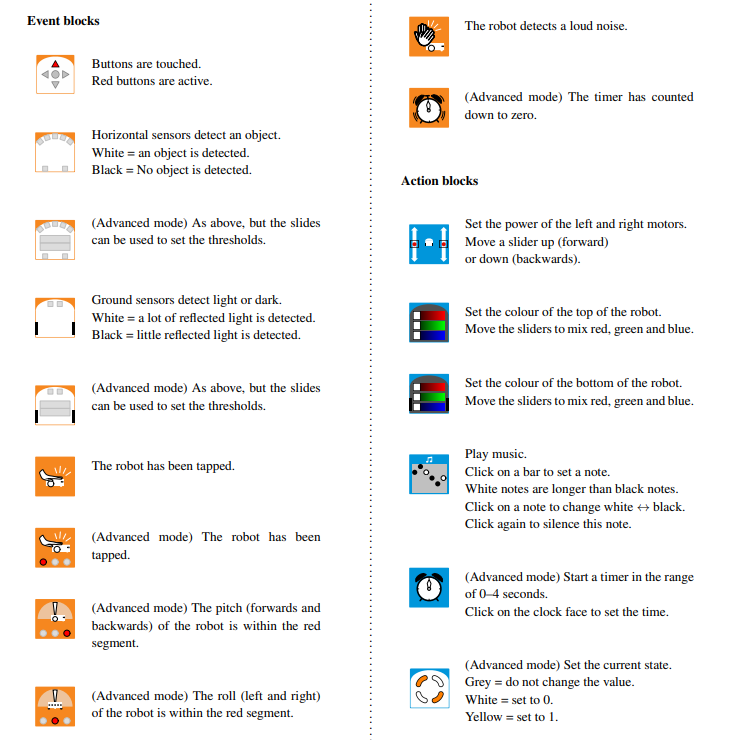
\includegraphics[width=\textwidth]{./VPL/Thymio_blocks}
  Thymio VPL Window
\end{center}

At first, the programming window will be empty of blocks, containing just a placeholder with empty slots. 
This placeholder is the base of every Thymio VPL program, it contains exactly one event block and one or more action block. 
This means that whenever the event of the event block happens then the set of actions added to this placeholder will occur at the same time. 
For example, with the following pair: \\
\begin{center}
  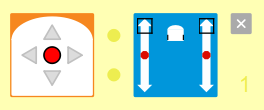
\includegraphics[scale=0.5]{./VPL/middlebtn_forward}\\
  Event and one Action relation
\end{center}

Both wheels are powered to the maximum when the middle button is pressed. But more than one action can be attributed to one event, 
to do so simply drag another action block onto the previous pair, notice that the same block cannot be used twice for the same event. 
Here we turned the lights on top and set them to a complete green:\\
\begin{center}
  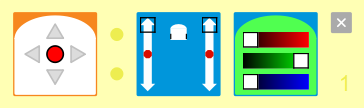
\includegraphics[scale=0.5]{./VPL/middlebtn_forward_green}\\
  Event and multiple Actions relation
\end{center}

The maximum amount of action blocks we can add to an event is four, but we can add as many event blocks to our program as we want. 
Let us add two more event blocks to allow the robot to turn:\\
\begin{center}
  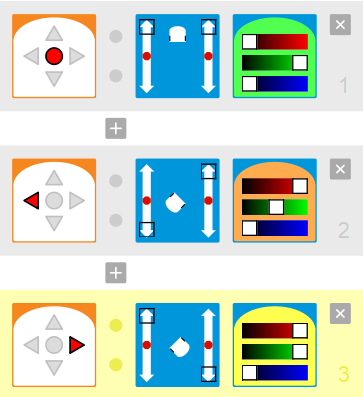
\includegraphics[scale=0.5]{./VPL/middlebtn_3E}\\
  Event and Actions relations
\end{center}

Now we have a basic behaviour, go straight with green lights when the middle button is pushed, turn left on itself with orange lights when the left button is pushed, 
and at last turn right on itself with yellow lights when the right button is pushed.\\

By clicking the button with a student as an icon we enable the advanced mode that gives us more possibilities for multiple blocks. It raises the amount of action block from four to six as well. \\

Let us refactor a bit the program from before, we will change the program by making the robot look left then right and starting over again using timers. 
To help us develop a more interesting program we have now access to a condition, a four led light on top of the robot, using this and the timer we can behave depending on the state of the robot. 
For example, hereafter the middle button was pressed a timer will start and after a short amount of time, it will light one particular led. 
Afterward, the event “timer elapsed” will be triggered but which pair should the program execute, turning right or turning left? 
Hence comes the use of the condition as we will execute the part of the program that corresponds to the state of the condition light. 
In this example, it will go back and forth between the two pairs: \\
\begin{center}
  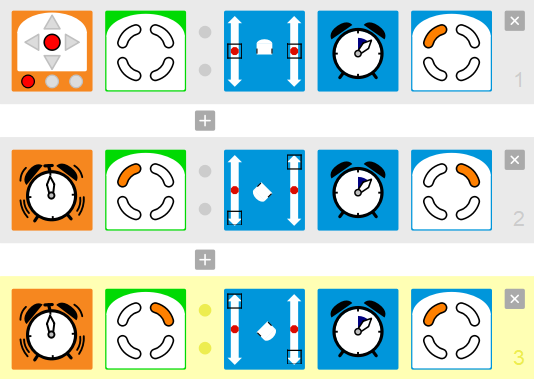
\includegraphics[scale=0.5]{./VPL/middlebtn_3E_adv}\\
  Advanced program
\end{center}

\section{Blockly 4 Thymio}

The second possibility is to use \texttt{Blockly4Thymio} which is an environment based on Blockly. Blockly was released in May 2012 and was initially a replacement for OpenBlocks for the \texttt{MIT App Inventor}. 
It is an open-source client-side library that allows its users to easily add a block-based visual programming language to an application or website. 
Blockly is not in itself a programming language but rather used to create one. Its design makes it flexible and it can support a large set of features. 
As it is a visual programming language, we find the same advantages as the first possibility, such for example applying programming principles with no regard towards syntactic error.
Blockly is among the growing and most used visual programming environments because of a few important features. First, it can export the code generated with the blocks to one of the five following programming languages, 
as a built-in feature, \texttt{JavaScript}, \texttt{Lua}, \texttt{Dart}, \texttt{Python}, and \texttt{PHP}, and can be enhanced for any textual programming languages. 
The block pool can be expanded from its base pool or even reduced depending on the needs. The blocks are not restrained to only basic tasks and can implement sophisticated programming tasks. 
And it has been translated in over forty languages, and as well right-to-left versions. \\

Blockly includes a set of pre-defined blocks that can be used to develop with more ease the wanted application. They are arranged into eight families:
\begin{description}
  \item [Logic:] Blocks with Boolean definition, equality check, and conditions.
  \item [Loop:] Blocks for loops.
  \item [Math:] Blocks for numbers, arithmetic operation, a few basic math functions (for example cos, sin, square root) and some mathematical constant (Pi).
  \item [Text:] Blocks to create text and text operations.
  \item [Lists:] Blocks to create lists and standard list operation (length, get the value).
  \item [Color:] Blocks with a color definition.
  \item [Variables:] Blocks to create variables, and to set/get their values.
  \item [Functions:] Blocks to create functions, with return value or not, and to call existing function.
\end{description}

Each block holds a pre-assigned shape, thus restraining its usage to certain situations as a "hidden" way to control the syntax. Their shapes are defined by the different connections with other blocks, 
both external and internal, while external blocks describe what happens after or before, the internals describe what happens during or what are the arguments, logic. 
Following is a basic variable block with three external connectors, and a math block with the value of one, with one connector, that is assigned to the \texttt{Count} variable (the blocks need to be assembled). \\
\begin{center}
  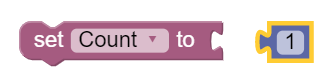
\includegraphics[scale=0.5]{./Blockly/basic_variable}\\
  Variable block
\end{center}

Using the same logic as above we created a \texttt{Limit} variable with the value of 5 to demonstrate the next example. 
The block used is from the logic family and test whether the \texttt{Count} variable is smaller or equal to the \texttt{Limit} as internal blocks. 
It can then be added to a loop, a function or other statements that needs logic.\\
\begin{center}
  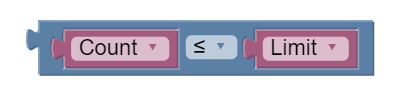
\includegraphics[scale=0.5]{./Blockly/basic_logic}\\
  Logic block
\end{center}

Added to the base that Blockly is for \texttt{Blockly4Thymio}, is a compilator that interpret and adapt the Blockly code directly into Aseba language, and an Aseba Framework. 
Let us once again follow the steps described in the “How does it works” section in order to start blockly-ing a little program with \texttt{Blockly4Thymio}. 
Note that it is possible to open the \texttt{Thymio Blockly} environment without going through the Thymio suite, and without any Thymio II connected (physically or simulated). 
To do so open the location of Thymio, the downloaded not the installed, and select thymio\textunderscore blockly, and then index.
The environment window that opens after choosing the Blockly option is split into four parts.
\begin{enumerate}
  \item A tool bar
  \item A programming window
  \item The category of blocks
  \item The program translated into AESL
\end{enumerate}

\begin{center}
  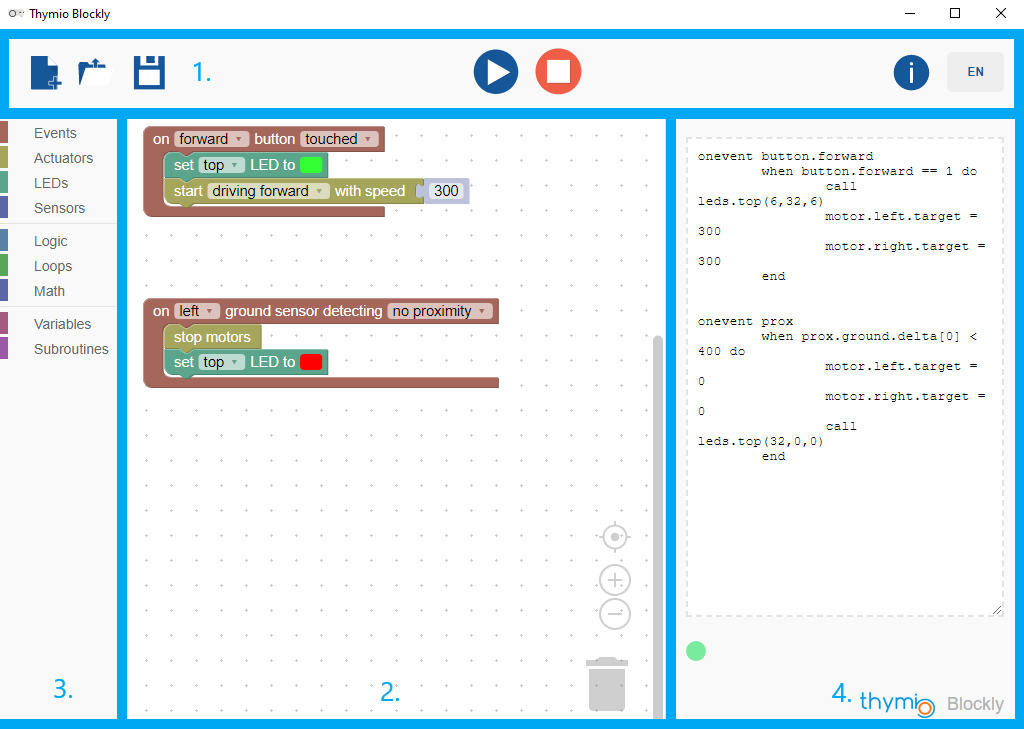
\includegraphics[scale=0.5]{./Blockly/blockly_window}\\
  Thymio Blockly window
\end{center}

The following figure demonstrates a simple program, once run the program listens to two different events. When the center button is pressed and when the front middle proximity sensor detects a wall. 
The first one will activate the two motors at the same speed, as to drive forward, and light the top LED to green. Whereas the second will stop the motors and turn the LED to red. \\
\begin{center}
  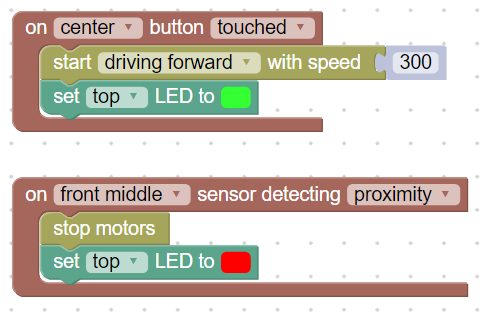
\includegraphics[scale=0.5]{./Blockly/forward_stop_wall}\\
  Basic program
\end{center}

Here we set a variable to act as a control if Thymio is moving or not. We then use this information into a test when we click the middle button, and we either move forward or stop according to the result. 
We added two other events for the right and left buttons that are responsible to turn the robot.
\begin{center}
  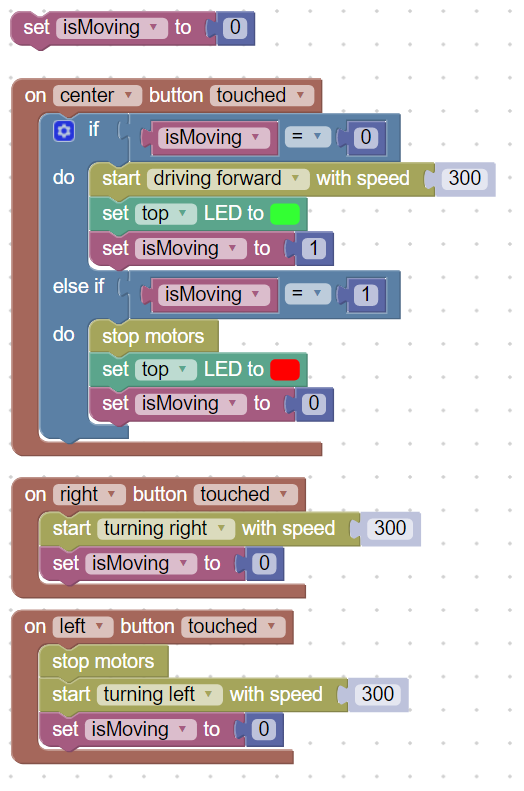
\includegraphics[scale=0.5]{./Blockly/advanced_program}\\
  More complex program
\end{center}

\section{Aseba}
\section{Scratch}

\chapter{Product Backlog}
\begin{longtable}{p{5mm}|p{2cm}|p{4cm}|p{1cm}|p{1cm}|p{1cm}|p{1cm}|p{15mm}}
  ID                     & Story Name & Story / Task Description & Priority & Est. Effort {[}h{]} & Update Effort {[}h{]} & Actual Effort{[}h{]} & Status                \\ \hline
  1 & Create Documentation & Develop and write the documentation & High & 16 & 16 & 16 & In-Progress \\ 
  2 & Set up the Environment & Setting up and configuring the development environment & High & 12 & 12 & 12 & Done \\ 
  3 & Basic Learning & Learning and training of the different technology used later on & High & 44 & 58 & 58 & Done \\ 
  4 & Develop Playgrounds & Create playgrounds and function to generate meshes & High & 40 & 48 & 48 & Done \\ 
  5 & Update Documentation & Update existing documentation & High & 60 &  &  & In-Progress \\
  6 & Architecture Implementation & Refactor the existing code into the designed architecture & High & 40 & 48 &  & In-Progress\\ 
  7 & Web Deployement & Deploy the application on a webserver & High & 16 & 12 & 12 & Done \\ 
  8 & Basic UI & Implement a basic UI & Low & 8 & 4 &  & In-Progress \\ 
  9 & Behaviour Pipeline & Create pipeline to take .aesl file and translate/compile it into behaviour in JavaScript for the Thymio II & High & 40 &  &  & To Do \\ 
  10 & Phyisics Implementation & Implementation of Collisions for threejs Meshes & High & 20 &  &  & To Do \\ 
  11 & Update Documentation & Update existing documentation & High & 20 &  &  & To Do \\ 
  12 & Enhanced UI & Enhancement of the current UI & Low &  &  &  & To Do \\ 
  13 & Customizable Playgrounds & Implementation of a playground creator for users & High &  &  &  & To Do \\ 
  14 & Update Documentation & Update existing documentation & High & 20 &  &  & To Do \\ 
  15 & Enhanced Behaviour Pipeline & Implement more sensors, action and event for Thymio II & High &  &  &  & To Do \\ 
  16 & Finish Documentation & Finish existing documentation & High &  &  &  & To Do \\
  17 & Prepare Defense & Prepare the defense & High &  &  &  & To Do \\ 
   &  &  & Total &  &  &  &  \\ 
\end{longtable}

\chapter{Sprint Backlog}
\section{First Sprint}
\textbf{2019-09-16 until 2019-10-07}
\begin{longtable}{p{5mm}|p{2cm}|p{4cm}|p{1cm}|p{1cm}|p{1cm}|p{1cm}|p{15mm}}
  ID                     & Story Name & Story / Task Description & Priority & Est. Effort {[}h{]} & Update Effort {[}h{]} & Actual Effort{[}h{]} & Status                \\ \hline
  1 & Create Documentation & Develop and write the documentation & High & 16 & 16 & 16 & Done \\ 
  1.1 & Template and Content & Choose a latex template and modify the content structure & High & 8 & 8 & 8 & Done \\ 
  1.2 & About Thymio & What is thymio and how does it work. & High & 8 & 8 & 8 & Done \\ 
  2 & Set up the Environment & Setting up and configuring the development environment & High & 12 & 12 & 12 & Done \\ 
  2.1 & GitHub & Create the project in GitHub and the Git environment & High & 4 & 4 & 4 & Done \\ 
  2.2 & Tools & Install Thymio Suite, NodeJS and download ThreeJS & High & 8 & 8 & 8 & Done \\ 
\end{longtable}

\section{Second Sprint}
\textbf{2019-10-07 until 2019-10-28}
\begin{longtable}{p{5mm}|p{2cm}|p{4cm}|p{1cm}|p{1cm}|p{1cm}|p{1cm}|p{15mm}}
  ID                     & Story Name & Story / Task Description & Priority & Est. Effort {[}h{]} & Update Effort {[}h{]} & Actual Effort{[}h{]} & Status                \\ \hline
  3 & Basic Learning & Learning and training of the different technology used later on & High & 44 & 58 & 58 & Done \\
  3.1 & threejs & Read documentation and examples, and practice & High & 16 & 20 & 20 & Done \\ 
  3.2 & JavaScript & Update and deepen knowledge  & High & 8 & 8 & 8 & Done \\ 
  3.3 & Thymio languages & Learning and using VPL, Blockly, Aseba and Scratch & Medium & 24 & 30 & 30 & Done \\ 
  4 & Develop Playgrounds & Create playgrounds and function to generate meshes & High & 40 & 48 & 48 & Done \\ 
  4.1 & Two Default Playgrounds & Generating two defalut playground to be choosen for the simulator & Medium & 12 & 12 & 12 & Done \\ 
  4.2 & Thymio Model & Create or load Thymio model & Medium & 4 & 4 & 4 & Done \\ 
  4.3 & Mesh Generation & Create function to generate meshes for the playgrounds & High & 24 & 32 & 32 & Done \\ 
  5 & Update Documentation & Update existing documentation & High & 60 & 12 &  & In-Progress \\
  5.1 & Four supported languages & Descibe and initiate to VPL, Blockly, Aseba and Scratch & High & 24 & 12 & {/} & In-Progress \\ 
\end{longtable}

\section{Third Sprint}
\textbf{2019-10-28 until 2019-11-15}
\begin{longtable}{p{5mm}|p{2cm}|p{4cm}|p{1cm}|p{1cm}|p{1cm}|p{1cm}|p{15mm}}
  ID                     & Story Name & Story / Task Description & Priority & Est. Effort {[}h{]} & Update Effort {[}h{]} & Actual Effort{[}h{]} & Status                \\ \hline
  5 & Update Documentation & Update existing documentation & High & 60 &  &  & In-Progress \\
  5.1 & Four supported languages & Descibe and initiate to VPL, Blockly, Aseba and Scratch & High & 24 & 24 &  & In-Progress \\ 
  5.2 & Backlogs & Create the Sprint and Project backlog & High & 12 & 8 & 16 & Done \\ 
  5.3 & Architecture & Create DCD, DM, PD, SD, SSD and proposition of architecture & High & 12 & 4 &  & In-Progress \\
  5.4 & User Stories & Formulate the User Stories & Medium & 4 & 4 & 4 & To Do \\ 
  5.5 & Risk Analysis & Create risk analysis & High & 8 &  &  & To Do \\ 
  6 & Architecture Implementation & Refactor the existing code into the designed architecture & High & 40 & 48 &  & In-Progress \\ 
  6.1 & Refactor Code & Refactor existing code into MVC Pattern & High & 20 & 44 & 44 & Done \\ 
  6.3 & Unit Testing & Write the JavaScript tests & High & 12 &  &  & To Do \\
  6.4 & JSDoc & Write the JavaScriptDoc & High & 8 & 4 &  & In-Progress \\ 
  7 & Web Deployement & Deploy the application on a webserver & High & 16 & 12 & 12 & Done \\ 
  7.1 & Virtual Machine Setup & Set up the Virtual machine & High & 8 & 4 & 4 & Done \\ 
  7.2 & WebServer & Create WebServer and publish it on bfh network & High & 8 & 8 & 8 & Done \\
  8 & Basic UI & Implement a basic UI & Low & 8 & 4 &  & In-Progress \\ 
  8.1 & Pages UI & Create three pages UI, one for each of the following index, simulation and creation pages & Low & 8 & 4 &  & In-Progress \\
\end{longtable}

\section{Fourth Sprint}
\textbf{2019-11-15 until 2019-12-09}
\begin{longtable}{p{5mm}|p{2cm}|p{4cm}|p{1cm}|p{1cm}|p{1cm}|p{1cm}|p{15mm}}
  ID                     & Story Name & Story / Task Description & Priority & Est. Effort {[}h{]} & Update Effort {[}h{]} & Actual Effort{[}h{]} & Status                \\ \hline
  9 & Behaviour Pipeline & Create pipeline to take .aesl file and translate/compile it into behaviour in JavaScript for the Thymio II & High & 40 &  &  & To Do \\ 
  10 & Phyisics Implementation & Implementation of Collisions for ThreeJS Meshes & High & 20 &  &  & To Do \\
  11 & Update Documentation & Update existing documentation & High & 20 &  &  & To Do \\ 
\end{longtable}

\section{Fifth Sprint}
\textbf{2019-12-09 until 2019-12-30}
\begin{longtable}{p{5mm}|p{2cm}|p{4cm}|p{1cm}|p{1cm}|p{1cm}|p{1cm}|p{15mm}}
  ID                     & Story Name & Story / Task Description & Priority & Est. Effort {[}h{]} & Update Effort {[}h{]} & Actual Effort{[}h{]} & Status                \\ \hline
  12 & Enhanced UI & Enhancement of the current UI & Low & 10 &  &  & To Do \\ 
  13 & Customizable Playgrounds & Implementation of a playground creator for users & High & 40 &  &  & To Do \\ 
  14 & Update Documentation & Update existing documentation & High & 20 &  &  & To Do \\ 
\end{longtable}

\section{Sixth Sprint}
\textbf{2019-12-30 until 2020-01-17}
\begin{longtable}{p{5mm}|p{2cm}|p{4cm}|p{1cm}|p{1cm}|p{1cm}|p{1cm}|p{15mm}}
  ID                     & Story Name & Story / Task Description & Priority & Est. Effort {[}h{]} & Update Effort {[}h{]} & Actual Effort{[}h{]} & Status                \\ \hline
  15 & Enhanced Behaviour Pipeline & Implement more sensors, action and event for Thymio II & High &  &  &  & To Do \\ 
  16 & Finish Documentation & Finish existing documentation & High &  &  &  & To Do \\
  16.1 & Create Video & Create the video file & High &  &  &  & To Do \\ 
  16.2 & Prepare Presentation Day & Create the poster and the presentation for the Presentation Day & High &  &  &  & To Do \\
  16.3 & Write in the Book & Write the page for the Book & High & 8 &  &  & To Do \\ 
  16.4 & Finish Writting Documentation & Terminate the writting part of the documentation & High &  &  &  & To Do \\ 
  16.5 & Prepare to Submit & Check spelling mistake, check images, print it, put the project on a USB stick & High &  &  &  & To Do\\ 
  17 & Prepare Defense & Prepare the defense & High &  &  &  & To Do \\ \hline
\end{longtable}

\chapter{Gantt Diagram}
\clearpage
\begin{center}
  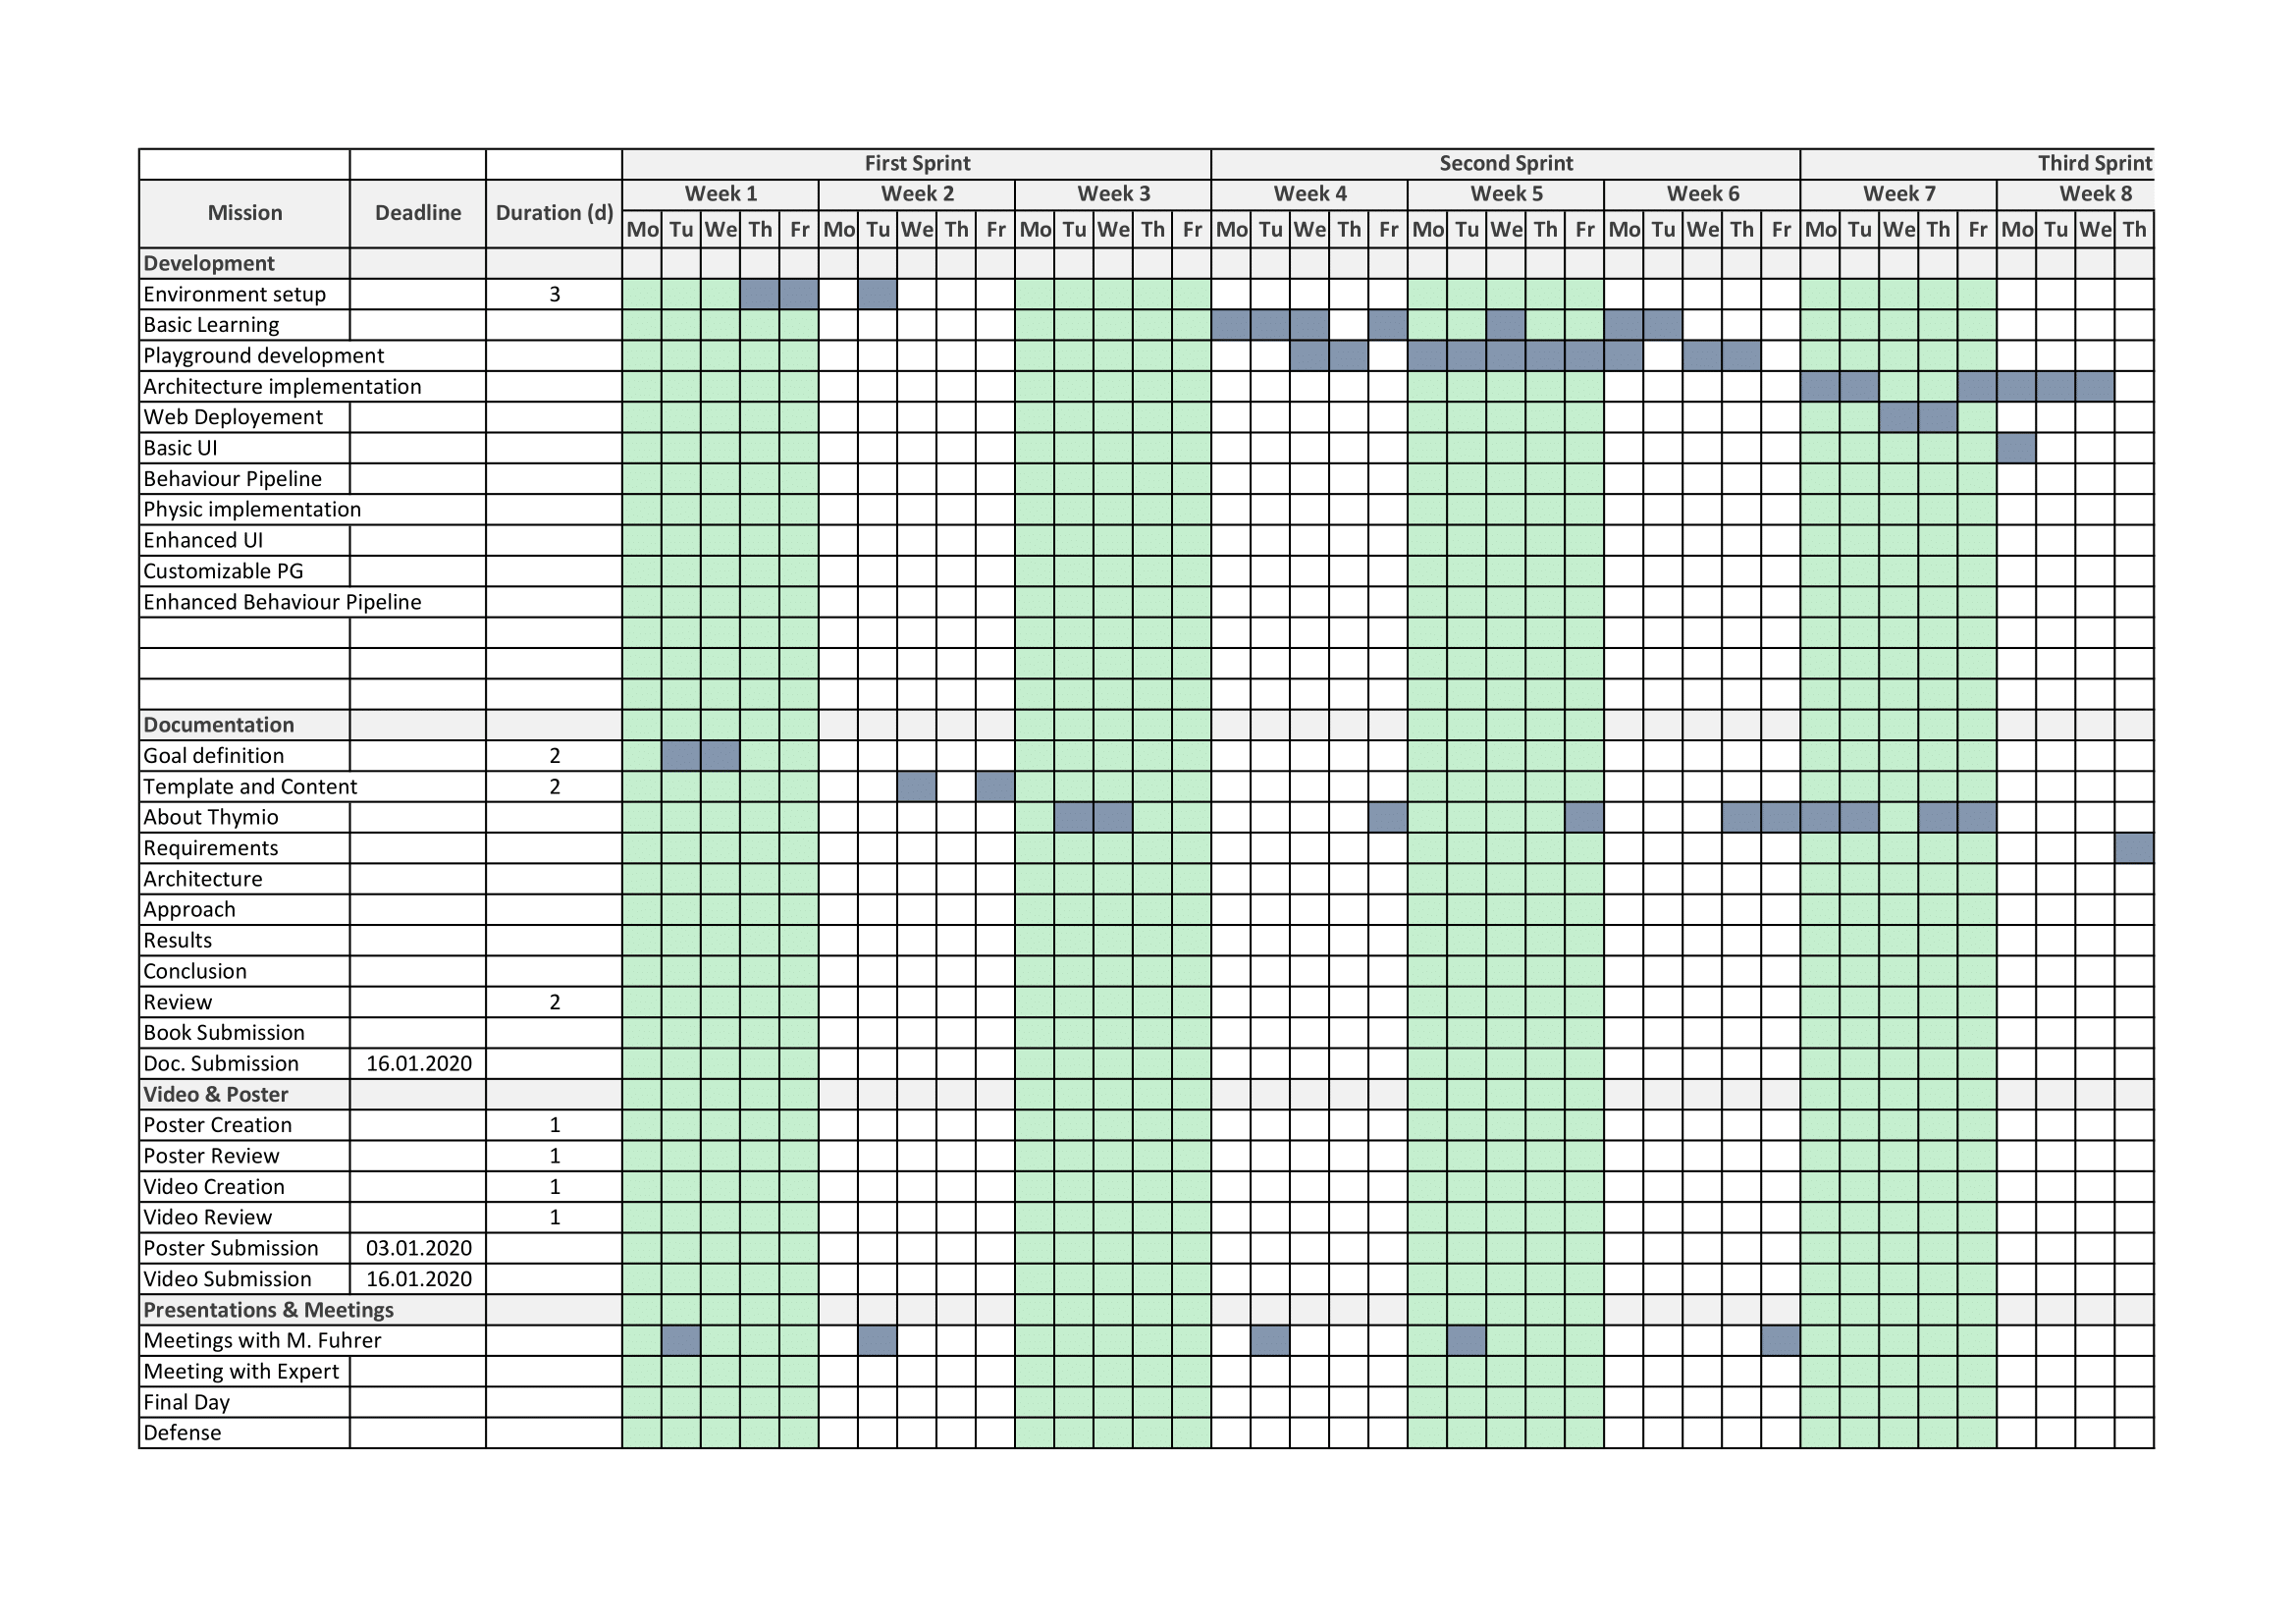
\includegraphics[scale = 0.28, angle=-90]{./Gantt-1}
\end{center}
\begin{center}
  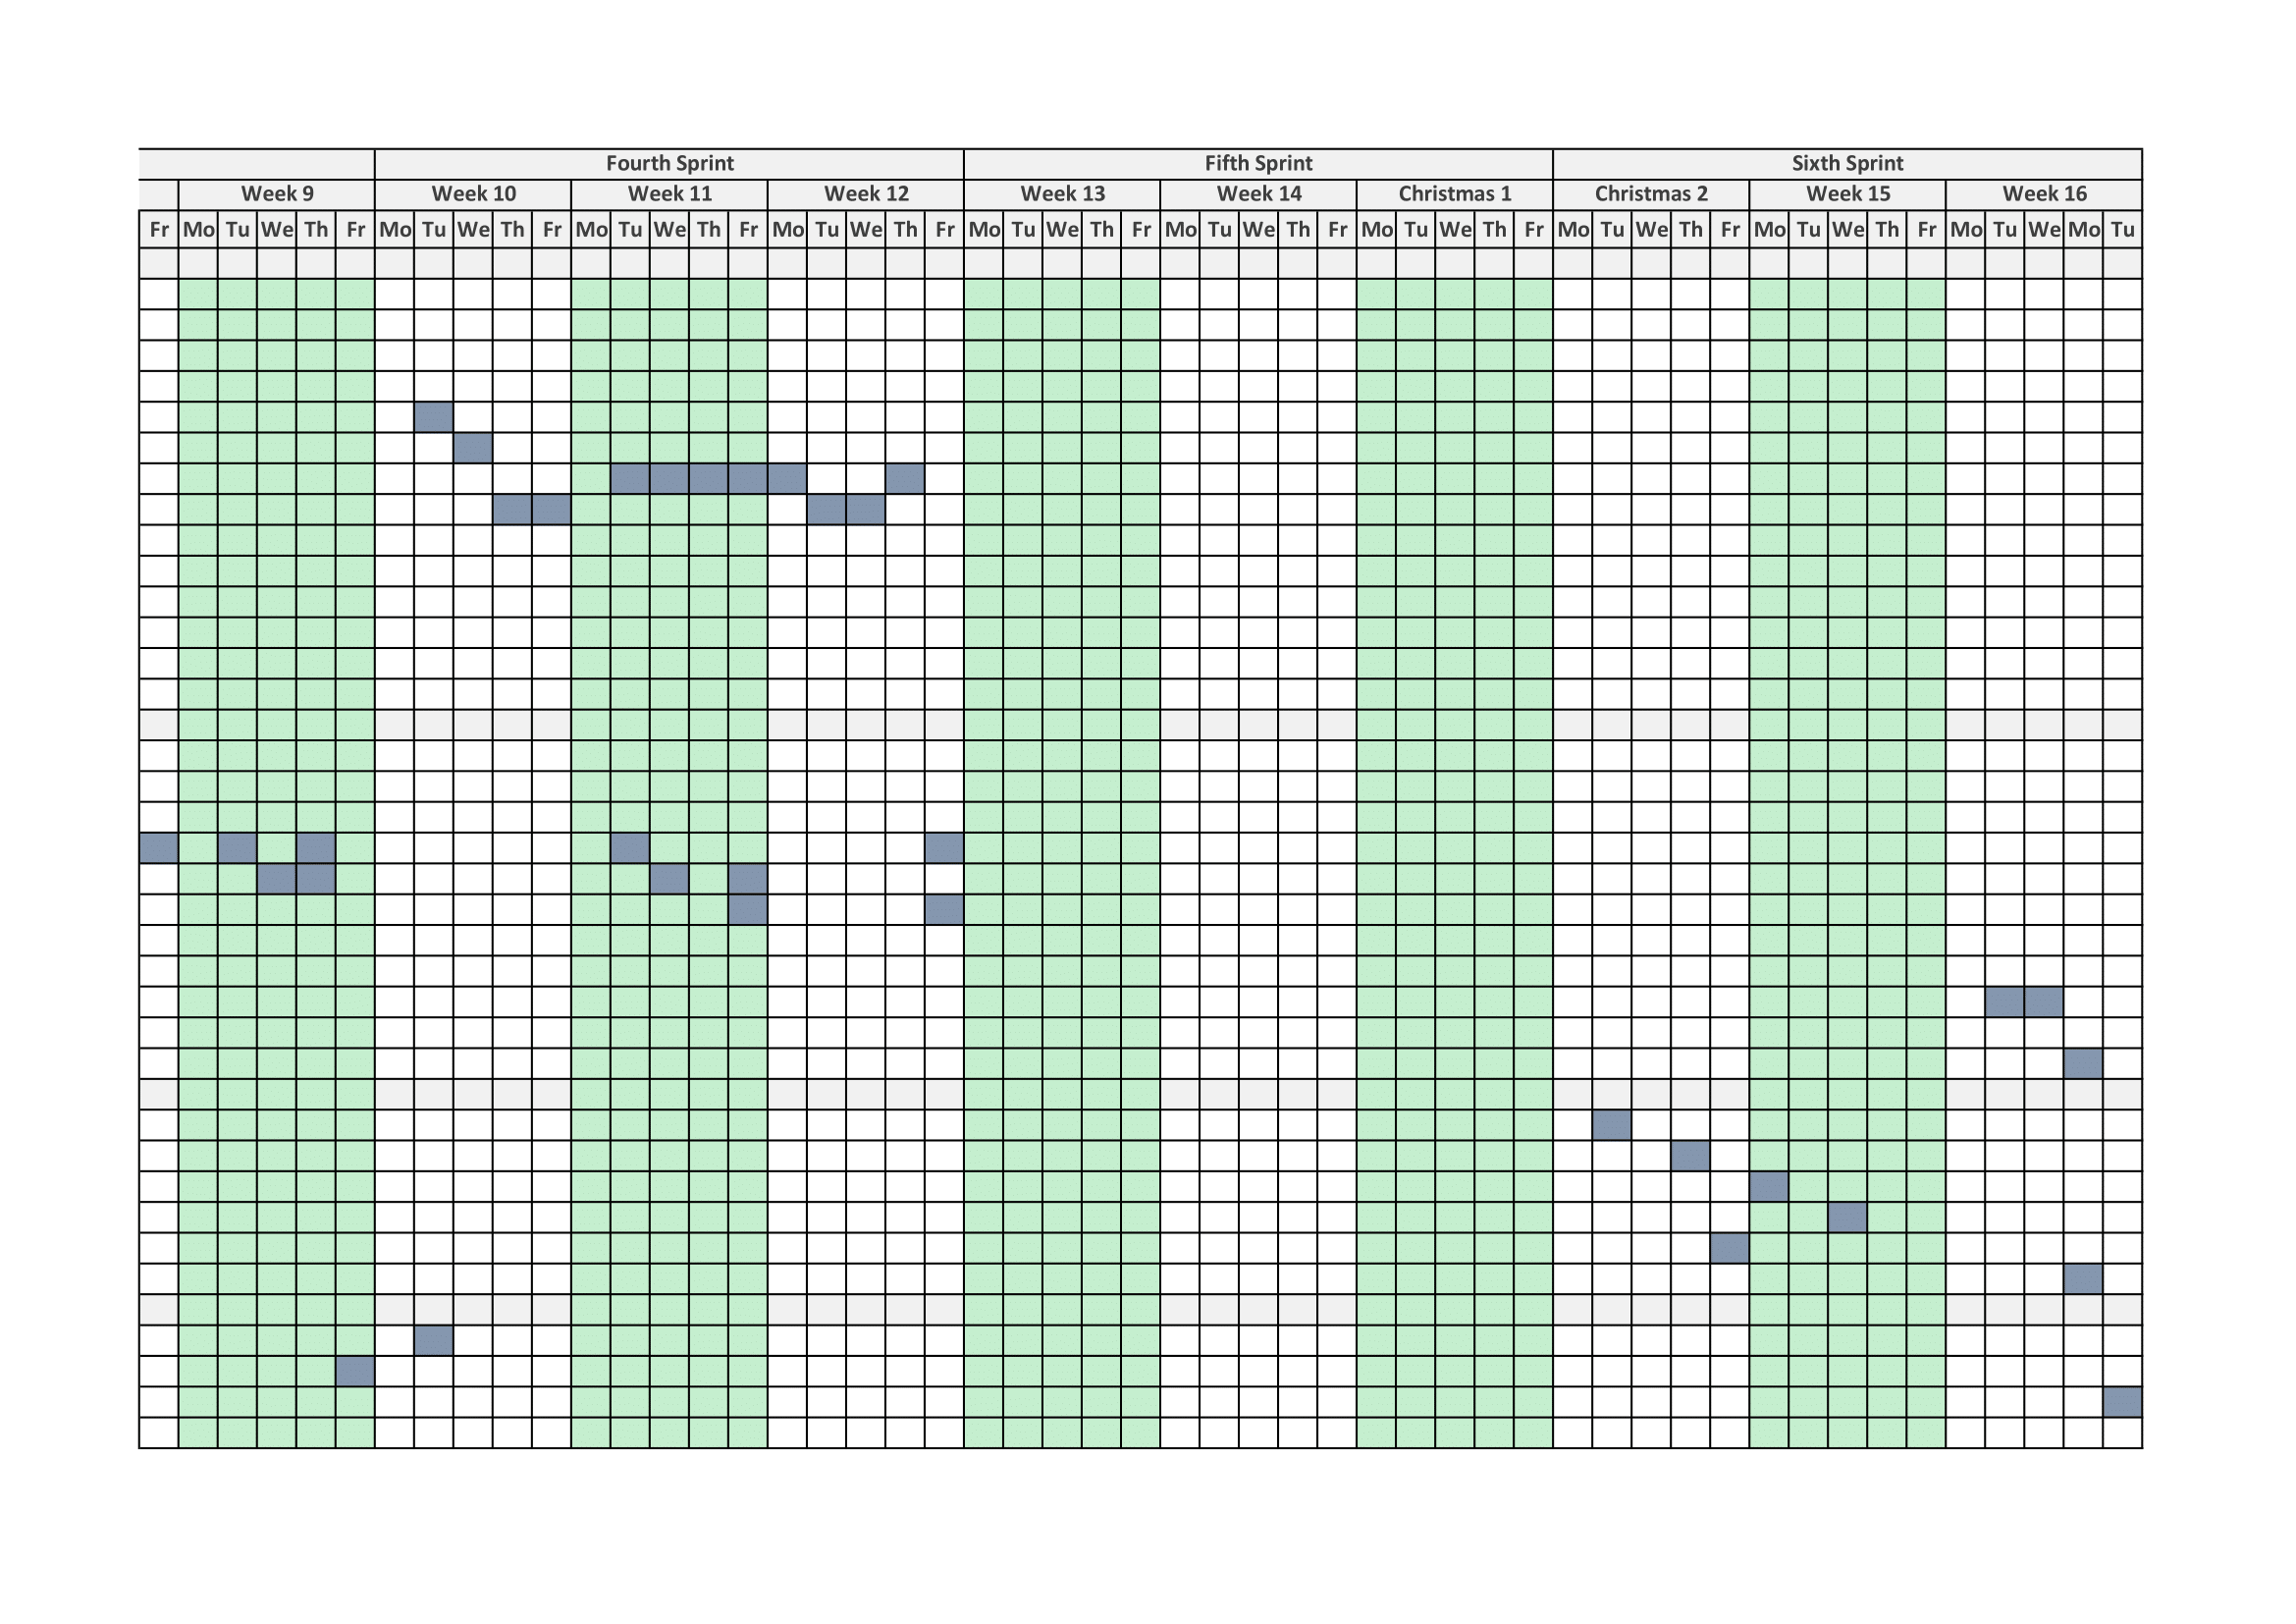
\includegraphics[scale = 0.28,  angle=-90]{./Gantt-2}
\end{center}
\clearpage

\chapter{Version control}

\chapter{Configuration}

\textbf{User information} \\
On demand.\\

\textbf{Access the Windows Virtual Machine}\\
\begin{center}
  \begin{tabular}{|c|c|c|}
    \hline
     & Linux WM -ssh & Windows VM - rdp \\
    \hline
    Windows & Putty & Remote Desktop Connection \\
    \hline
    Linux & terminal & Remmina \\
    \hline
    MacOS & terminal & Microsoft Remote Desktop \\
    \hline
  \end{tabular}
\end{center}

See link bellow for more information and links. (It requires to be inside the bfh networkd to access it)
\url{https://intranet.bfh.ch/TI/fr/Studium/Bachelor/Informatik/Tools/VMsHowto/Pages/default.aspx?k=vm}

\textbf{First Configuration of XAMPP}\\
The configuration of XAMPP is very basic. The steps done during the setup of the IIS Manager at \ref{webserver}, concerning forwarding and firewall, should still be followed. First we need to download and install it, it can be found under this link : \url{https://www.apachefriends.org/index.html} . Afterward it is needed to travel through the folder of the application until the folder 
\texttt{htdocs}. There was stored the default placeholder files, we put them into a new default folder and instead added our content in this folder. Do not forget to take the .webconfig file from the \ref{webserver} section.

\chapter{Meetings}
\begin{tabular}{ | m{3cm} | m{10cm} | }
  \hline
  Date & Content \\
  \hline
  17.09.2019 & \textbf{Kick Off meeting}\\
  & - Documentation/Management\\
  & - Technology to use : ThreeJS and Typescript\\
  & - Setting up the goals\\
  \hline
  24.09.2019 & \textbf{Second meeting} \\
  & - Documentation language : English \\
  & - Thymio model \\
  & - Base talk about riks management \\
  \hline
  08.10.2019 & \textbf{Third meeting}\\
  & Workplace\\
  & - Discussion on the choice of Windows as the Virtual Machine \\
  & - Create a configuration file with the information of the VM \\
  & - And an architecture proposal \\
  \hline
  15.10.2019 & \textbf{Fourth meeting} \\
  & - Which shapes and meshes should the user be able to create for his own custom playground \\
  & - Problems with webserver, has to be accessible from outside the vm, so maybe switching from windosw to linux \\
  & - Talk about the problem of thymio suite, that is the software allows the user to create programs only if a physical or a simulated one is plugged in \\
  \hline
  25.10.2019 & \textbf{Fifth meeting} \\
  & - Discussed using a Finite state machine to handle the events, but it may be too rigid so a non-deterministic finite state machine was the possible solution we came with \\
  & - First little talk about the meeting with the expert, report\\
  \hline
  19.11.2019 & \textbf{Sixth meeting} \\
  & \\
  \hline
\end{tabular}

\chapter{Problems encountered}
\begin{itemize}
  \item javascript not refreshing properly due to cache -> disable cache
  \item 3d Model not loaded on the webserver -> first tried to change the directory, then mixed two solution. 
        Had to create a web.config file and add file extension for .mtl and .obj.
        https://stackoverflow.com/questions/41245938/web-server-cannot-find-mtl-file
        https://stackoverflow.com/questions/16097580/three-js-loading-obj-error-in-azure-but-not-locally
  \item shadow not rendering on plane of all playgrounds
  \item javascript file not found on server, net::ERR\textunderscore ABORTED 404 (Not Found) => first solution (working partially) was to add a IIS\textunderscore IUSRS.
  \item Thymio Blockly has trouble loading saved files. Using the software I wasn't able to load any .aesl file previously created with it, but I could load them if I used the index.html one.
  \item Thymio model not always loading correctly -> Load one at the start of the page and reset its position/rotation upon change of playground.
  \item problem with dat.gui, it was creating a new creator view so the creator wasn't accessible. Decided to use html buttons instead
  \item c++ to javascript
\end{itemize}

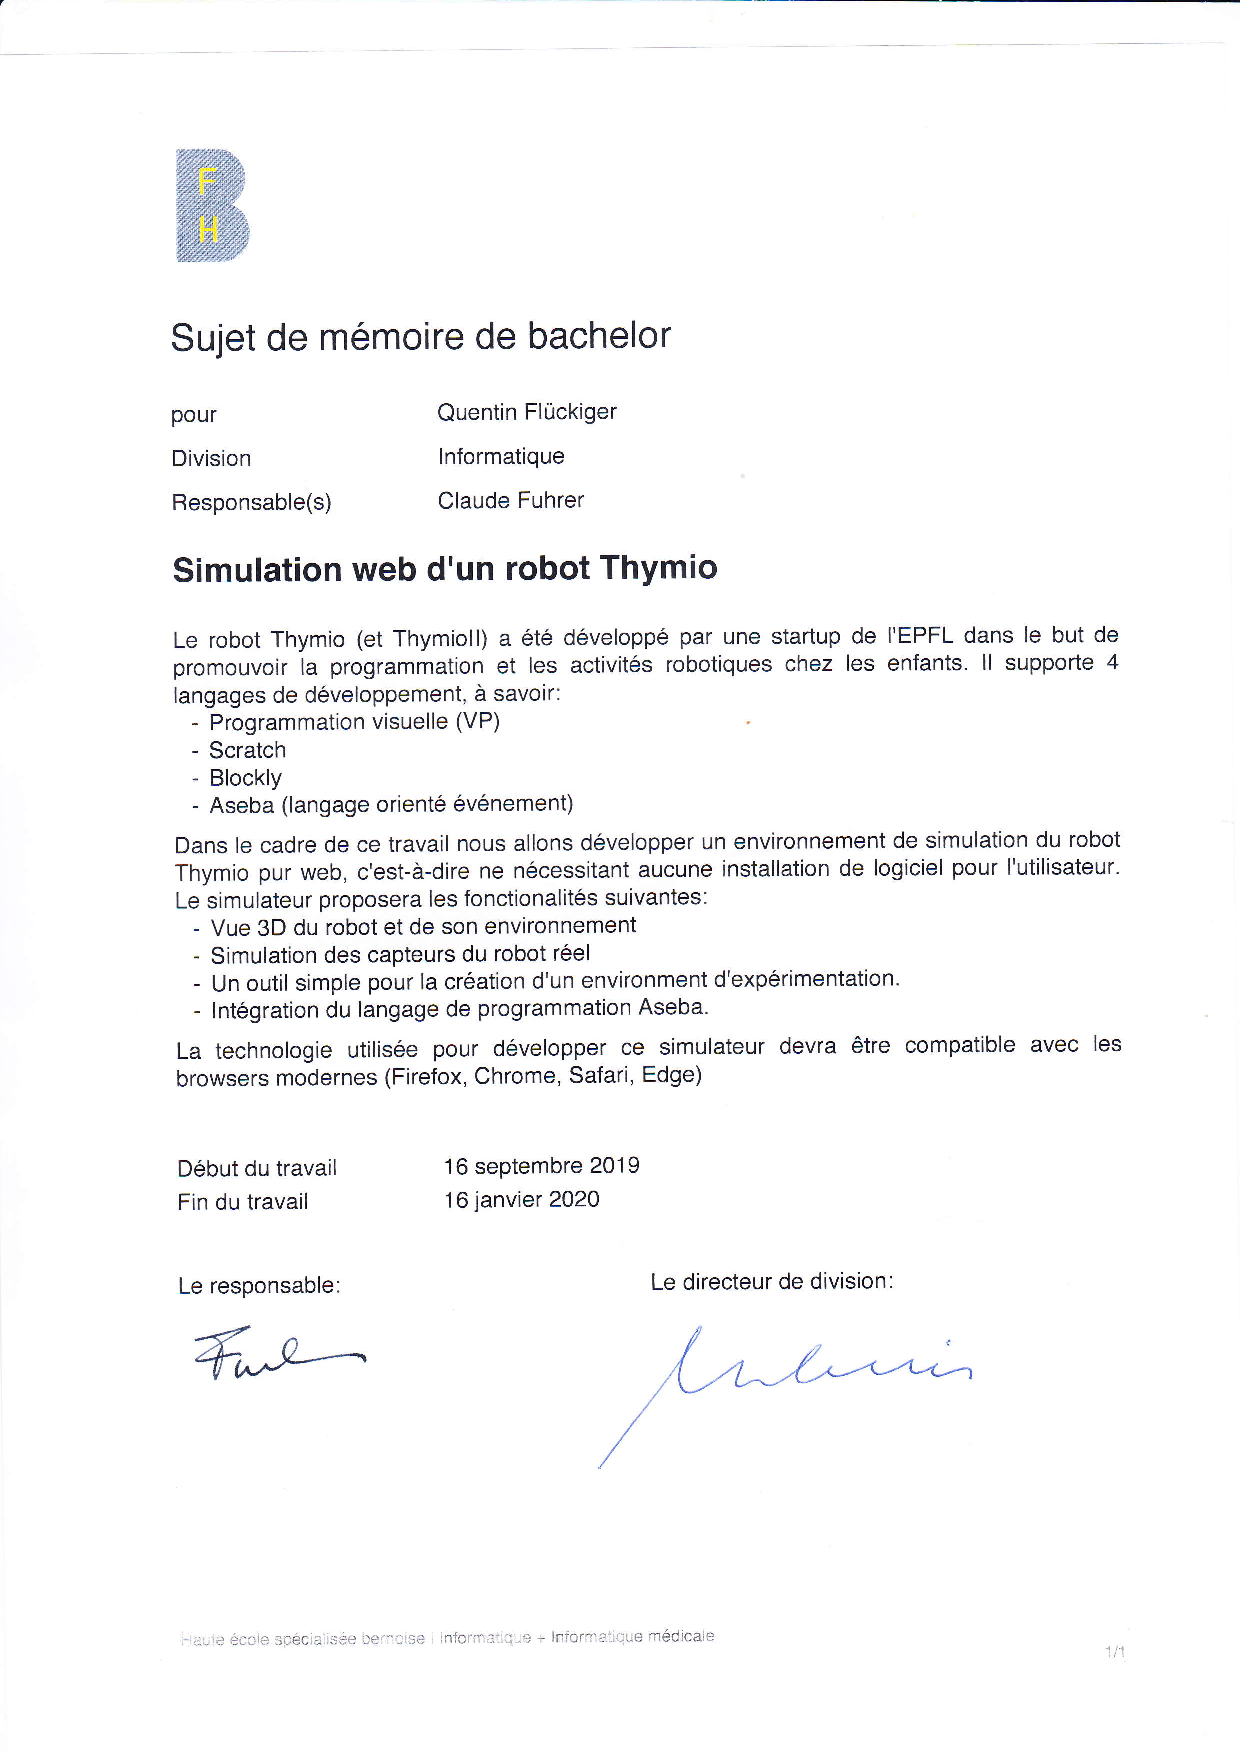
\includegraphics[width=\textwidth]{./bachelor_quentin.pdf}

%% Print the bibibliography and add the section to the table of content
\printbibliography[heading=bibintoc]

\end{document}
